\documentclass{eieproyecto}
\usepackage{gensymb}
\usepackage{epstopdf}
\usepackage{verbatim}
\usepackage{listings}
\usepackage{color}
\usepackage{subcaption}
\definecolor{dkgreen}{rgb}{0,0.6,0}
\definecolor{gray}{rgb}{0.5,0.5,0.5}
\definecolor{mauve}{rgb}{0.58,0,0.82}

\definecolor{lightgray}{rgb}{0.95, 0.95, 0.95}
\definecolor{darkgray}{rgb}{0.4, 0.4, 0.4}
\definecolor{purple}{rgb}{0.65, 0.12, 0.82}
\definecolor{editorGray}{rgb}{0.95, 0.95, 0.95}
\definecolor{editorOcher}{rgb}{1, 0.5, 0} % #FF7F00 -> rgb(239, 169, 0)
\definecolor{editorGreen}{rgb}{0, 0.5, 0} % #007C00 -> rgb(0, 124, 0)
\usepackage[table,xcdraw]{xcolor}
\usepackage{upquote}
\usepackage{pgfgantt}
% CSS

%\usepackage{bera}% optional: just to have a nice mono-spaced font
\usepackage{xcolor}
\usepackage{float}
\restylefloat{table}

\colorlet{punct}{red!60!black}
\definecolor{background}{HTML}{EEEEEE}
\definecolor{delim}{RGB}{20,105,176}
\colorlet{numb}{magenta!60!black}

\lstdefinelanguage{json}{
	basicstyle=\normalfont\ttfamily,
	numbers=left,
	numberstyle=\scriptsize,
	stepnumber=1,
	numbersep=8pt,
	showstringspaces=false,
	breaklines=true,
	frame=lines,
	backgroundcolor=\color{background},
	literate=
	*{0}{{{\color{numb}0}}}{1}
	{1}{{{\color{numb}1}}}{1}
	{2}{{{\color{numb}2}}}{1}
	{3}{{{\color{numb}3}}}{1}
	{4}{{{\color{numb}4}}}{1}
	{5}{{{\color{numb}5}}}{1}
	{6}{{{\color{numb}6}}}{1}
	{7}{{{\color{numb}7}}}{1}
	{8}{{{\color{numb}8}}}{1}
	{9}{{{\color{numb}9}}}{1}
	{:}{{{\color{punct}{:}}}}{1}
	{,}{{{\color{punct}{,}}}}{1}
	{\{}{{{\color{delim}{\{}}}}{1}
	{\}}{{{\color{delim}{\}}}}}{1}
	{[}{{{\color{delim}{[}}}}{1}
	{]}{{{\color{delim}{]}}}}{1},
}


\lstdefinelanguage{CSS}{
	keywords={color,background-image:,margin,padding,font,weight,display,position,top,left,right,bottom,list,style,border,size,white,space,min,width, transition:, transform:, transition-property, transition-duration, transition-timing-function},	
	sensitive=true,
	morecomment=[l]{//},
	morecomment=[s]{/*}{*/},
	morestring=[b]',
	morestring=[b]",
	alsoletter={:},
	alsodigit={-}
}

% JavaScript
\lstdefinelanguage{JavaScript}{
	morekeywords={typeof, new, true, false, catch, function, return, null, catch, switch, var, if, in, while, do, else, case, break},
	morecomment=[s]{/*}{*/},
	morecomment=[l]//,
	morestring=[b]",
	morestring=[b]'
}

\lstdefinelanguage{HTML5}{
	language=html,
	sensitive=true,	
	alsoletter={<>=-},	
	morecomment=[s]{<!-}{-->},
	tag=[s],
	otherkeywords={
		% General
		>,
		% Standard tags
		<!DOCTYPE,
		</html, <html, <head, <title, </title, <style, </style, <link, </head, <meta, />,
		% body
		</body, <body,
		% Divs
		</div, <div, </div>, 
		% Paragraphs
		</p, <p, </p>,
		% scripts
		</script, <script,
		% More tags...
		<canvas, /canvas>, <svg, <rect, <animateTransform, </rect>, </svg>, <video, <source, <iframe, </iframe>, </video>, <image, </image>
	},
	ndkeywords={
		% General
		=,
		% HTML attributes
		charset=, src=, id=, width=, height=, style=, type=, rel=, href=,
		% SVG attributes
		fill=, attributeName=, begin=, dur=, from=, to=, poster=, controls=, x=, y=, repeatCount=, xlink:href=,
		% CSS properties
		margin:, padding:, background-image:, border:, top:, left:, position:, width:, height:,
		% CSS3 properties
		transform:, -moz-transform:, -webkit-transform:,
		animation:, -webkit-animation:,
		transition:,  transition-duration:, transition-property:, transition-timing-function:,
	}
}

\lstset{%
	% General design
	backgroundcolor=\color{editorGray},
	basicstyle={\small\ttfamily},   
	frame=l,
	% line-numbers
	xleftmargin={0.75cm},
	numbers=left,
	stepnumber=1,
	firstnumber=1,
	numberfirstline=true,	
	% Code design
	identifierstyle=\color{black},
	keywordstyle=\color{blue}\bfseries,
	ndkeywordstyle=\color{editorGreen}\bfseries,
	stringstyle=\color{editorOcher}\ttfamily,
	commentstyle=\color{darkgray}\ttfamily,
	% Code
	language=HTML5,
	alsolanguage=JavaScript,
	alsodigit={.:;},	
	tabsize=2,
	showtabs=false,
	showspaces=false,
	showstringspaces=false,
	extendedchars=true,
	breaklines=true,
	% German umlauts
	literate=%
	{Ö}{{\"O}}1
	{Ä}{{\"A}}1
	{Ü}{{\"U}}1
	{ß}{{\ss}}1
	{ü}{{\"u}}1
	{ä}{{\"a}}1
	{ö}{{\"o}}1
}

%Packages
\usepackage{xspace}
\usepackage{color}

%Colours
%ucr
\definecolor{celesteUCR}{RGB}{65,173,231}
\definecolor{amarilloUCR}{RGB}{249,234,100}
\definecolor{verdeUCR}{RGB}{81,186,69}
%
%tum
\definecolor{blueTUM}{RGB}{0,105,178}
%
\definecolor{redPRIS}{RGB}{180,0,0}
\definecolor{yellowPRIS}{RGB}{240,230,170}
\definecolor{grayPRIS}{RGB}{90,100,140}
\definecolor{blackPRIS}{RGB}{0,0,0}
%
\definecolor{prisred}{RGB}{180,0,0}
\definecolor{prisgrey}{RGB}{180,150,150}
\definecolor{darkgrey}{RGB}{50,60,70}
\definecolor{lightgrey}{RGB}{150,150,150}
\definecolor{labgrey}{RGB}{90,100,140}
\definecolor{labyellow}{RGB}{240,230,170}
\definecolor{prisgray}{RGB}{50,60,70}
\definecolor{prisblack}{RGB}{0,0,0}
\definecolor{prisblue}{RGB}{40,65,140}
\definecolor{ace1}{RGB}{0,150,215}
\definecolor{ace2}{RGB}{0,50,70}
\definecolor{ribBlue}{RGB}{0,100,150}

\definecolor{pris}{RGB}{180,0,0}
\definecolor{prisblue}{RGB}{40,65,140}
% \definecolor{prisgray}{RGB}{107,107,107}
\definecolor{labyellow}{RGB}{240,230,170}
\definecolor{lightgrey}{RGB}{150,150,150}

%Teknovae colors
\definecolor{teknovaeBlack}{RGB}{0,0,0}
\definecolor{teknovaeOrange}{RGB}{255,139,51}
\definecolor{teknovaeGreen}{RGB}{3,204,0}
\definecolor{teknovaeBlue}{RGB}{65,26,255}
%
\definecolor{blackTKN}{RGB}{0,0,0}
\definecolor{redTKN}{RGB}{255,139,51}
\definecolor{greenTKN}{RGB}{3,204,0}
\definecolor{blueTKN}{RGB}{65,26,255}

%Fonts
\DeclareFontFamily{T1}{pbk}{}
\DeclareFontFamily{T1}{pbks}{}
\DeclareFontShape{T1}{pbk}{m}{n}{<->s*pbkl}{}
\DeclareFontShape{T1}{pbks}{m}{n}{<->s*[0.7]pbkl}{}

%Names
\newcommand{\prislab}{{\fontfamily{pbk}\selectfont\textcolor{prisred}{PR}\textcolor{prisblack}{IS}}{\fontfamily{pbks}\selectfont\textcolor{prisgray}{-LAB}}\xspace}
\newcommand{\pris}{Pattern Recognition and Intelligent Systems Laboratory\xspace}
\newcommand{\prises}{Laboratorio de Investigación en Reconocimiento de Patrones y Sistemas Inteligentes\xspace}
\newcommand{\prisfull}{\prislab: \pris}
\newcommand{\prisfulles}{\prislab: \prises}

\definecolor{core1}{RGB}{75,95,115}
\definecolor{core2}{RGB}{220,60,60}
\newcommand{\core}{{\fontfamily{bookman}\sc \textcolor{core1}{C}\textcolor{core2}{o}\textcolor{core1}{re}}\xspace}

\definecolor{excess1}{RGB}{33,180,168}
\definecolor{excess2}{RGB}{190,0,60}
\newcommand{\excess}{{\fontfamily{bookman}\sc \textcolor{excess1}{E}\textcolor{excess2}{x}\textcolor{excess1}{cess}}\xspace}

\definecolor{essence1}{RGB}{90,140,50}
\definecolor{essence2}{RGB}{124,222,50}
\newcommand{\essence}{{\fontfamily{bookman}\sc \textcolor{essence1}{E}\textcolor{essence2}{ss}\textcolor{essence1}{ence}}\xspace}

\newcommand{\bend}{{\fontfamily{bookman}\sc \textcolor{excess2}{B}\textcolor{excess1}{e}\textcolor{excess1}{nd}}\xspace}
\newcommand{\hint}{{\fontfamily{bookman}\sc \textcolor{essence1}{H}\textcolor{essence2}{int}}\xspace}

% PRIS-Lab
% \newcommand{\pris}{Pattern Recognition and Intelligent Systems Laboratory\xspace}
% \newcommand{\prislab}{{\fontfamily{bookman}\sc\textcolor{prisred}{PR}\textcolor{black}{IS\textcolor{prisgray}{-lab}}}\xspace}
% \newcommand{\bcrn}{{\fontfamily{bookman}\sc\textcolor{prisred}{PR}\textcolor{black}{IS\textcolor{prisgray}{-lab}}}\xspace}
% \newcommand{\prisfull}{{\fontfamily{bookman}\sc\prislab}: \pris}
% \newcommand{\prislabfull}{\sc Laboratorio de Investigación en\\\textcolor{redPRIS}{Reconocimiento de Patrones}\\y Sistemas Inteligentes}
\newcommand{\aprs}{{\fontfamily{bookman}\sc APRS}\xspace}
\newcommand{\aprsfull}{{\fontfamily{bookman}\sc\aprs}: Advanced Pattern Recognition System\xspace}
\newcommand{\aprsfulles}{{\fontfamily{bookman}\sc\aprs}: Sistema Avanzado de Reconocimiento de Patrones\xspace}
%
\newcommand{\prissem}{{\fontfamily{bookman}\sc\textcolor{prisred}{PR}\textcolor{black}{IS\textcolor{black}{-Seminar}}}\xspace}
\newcommand{\coloquio}{\textit{Coloquio de Investigación}\xspace}
\newcommand{\ace}{{\fontfamily{bookman}\sc\textcolor{ace1}{A}\textcolor{ace2}{ce}}\xspace}

\newcommand{\sura}{{\fontfamily{bookman}\sc\textcolor{prisred}{S}\textcolor{black}{u}\textcolor{prisblue}{r}\textcolor{prisgray}{á}}\xspace}
\newcommand{\boknama}{{\fontfamily{bookman}\sc Boknama}\xspace}
\newcommand{\iriria}{{\fontfamily{bookman}\sc Iriria}\xspace}

%Networks
\newcommand{\rib}{{\fontfamily{bookman}\sc\textcolor{ribBlue}{RIB}}\xspace}
\newcommand{\ribfull}{\rib: Red de Investigación en Biocomputación\xspace}
\newcommand{\bcrn}{{\fontfamily{bookman}\sc\textcolor{ribBlue}{BcRN}}\xspace}
\newcommand{\bcrnfull}{\bcrn: Biocomputing Research Network\xspace}

\newcommand{\rider}{{\fontfamily{bookman}\sc \textcolor{orange!80!black}{Rider}}\xspace}
\newcommand{\riderfull}{\rider: Red de Investigación y Desarrollo en Eficiencia Energética y Tecnologías en Energía Renovable\xspace}

\newcommand{\ricc}{{\fontfamily{bookman}\sc \textcolor{red!80!black}{R}\textcolor{green!80!black}{I}\textcolor{blue!80!black}{C}\textcolor{prisgray}{C}}\xspace}
\newcommand{\riccfull}{\ricc: Red de Investigación en Computación Científica\xspace}
\newcommand{\scrn}{{\fontfamily{bookman}\sc \textcolor{red!80!black}{S}\textcolor{green!80!black}{C}\textcolor{blue!80!black}{R}\textcolor{prisgray}{N}}\xspace}
\newcommand{\scrnfull}{\scrn: Scientific Computing Research Network\xspace}

%Institutions
\newcommand{\arcoslab}{ARCOS-LAB\xspace}
\newcommand{\arcoslabfull}{\arcoslab: Autonomous Robots and Cognitive Systems Laboratory\xspace}

\newcommand{\clcar}{CLCAR\xspace}
\newcommand{\clcarfull}{\clcar: Conferencia Latinoamericana de Computación de Alto Rendimiento\xspace}

\newcommand{\nsf}{{\fontfamily{bookman}\sc NSF}\xspace}
\newcommand{\nsffull}{\nsf: National Science Foundation\xspace}

\newcommand{\conare}{{\fontfamily{bookman}\sc CONARE}\xspace}
\newcommand{\conarefull}{\conare: Consejo Nacional de Rectores\xspace}

\newcommand{\cenat}{{\fontfamily{bookman}\sc CeNAT}\xspace}
\newcommand{\cenatfull}{\cenat: Centro Nacional de Alta Tecnología\xspace}

\newcommand{\cnca}{{\fontfamily{bookman}\sc CNCA}\xspace}
\newcommand{\cncafull}{\cnca: Co-laboratorio Nacional de Computación Avanzada\xspace}
\newcommand{\cadejos}{{\fontfamily{bookman}\sc\textcolor{black}{cadejos}}\xspace}

\newcommand{\ictp}{ICTP: International Centre for Theoretical Physics\xspace}


\newcommand{\ucr}{Universidad de Costa Rica\xspace}
\newcommand{\eie}{Escuela de Ingeniería Eléctrica\xspace}
\newcommand{\fing}{Facultad de Ingeniería\xspace}

\newcommand{\towhom}{To Whom it May Concern\xspace}
\newcommand{\aquien}{A Quien Corresponda\xspace}

\newcommand{\fourVidTags}{\emph{4vid}\textit{Tags}\xspace}



%Conferences
\newcommand{\ines}{17th IEEE International Conference on Intelligent Engineering Systems -- INES\xspace}
\newcommand{\cinti}{14th IEEE International Symposium on Computational Intelligence and Informatics -- CINTI\xspace}
\newcommand{\sami}{IEEE International Symposium on Applied Machine Intelligence and Informatics -- SAMI\xspace}

%People
\newcommand{\juanD}{Juan Marcos Delgado Zumbado, MLE\xspace}
\newcommand{\juanDjob}{Director}
\newcommand{\juanDwho}{Estimado Sr. Delgado}

\newcommand{\lauraR}{Laura Robles Loaiza, Licda.\xspace}
\newcommand{\lauraRjob}{Unidad de adquisiciones, \os}
\newcommand{\lauraRwho}{Estimada Sra. Robles}

\newcommand{\yamilethF}{Yamileth Figueroa Barahona, MBA.\xspace}
\newcommand{\yamilethFjob}{Directora de la Dirección Financiera, Rectoría\xspace}
\newcommand{\olgaC}{Olga Cordero Quirós\xspace}
\newcommand{\olgaCjob}{Gestora de la Dirección Financiera, Rectoría\xspace}
\newcommand{\electrizarte}{ElectrizArte\xspace}

\newcommand{\oaice}{OAICE\xspace}
\newcommand{\oaicefull}{\oaice: Oficina de Asuntos Internacionales y Cooperación Externa\xspace}
\newcommand{\oaicename}{Oficina de Asuntos Internacionales y Cooperación Externa\xspace}

\newcommand{\julietaC}{Dra. Julieta Carranza Velázquez\xspace}
\newcommand{\julietaCjob}{Directora \oaice\xspace}
\newcommand{\julietaCwho}{Estimada Dra. Carranza\xspace}

\newcommand{\walterM}{Dr. Walter Marín Méndez\xspace}
\newcommand{\walterMjob}{Subdirector \oaicename\xspace}
\newcommand{\walterMwho}{Estimado Dr. Marín\xspace}

\newcommand{\fatimaA}{Fátima Acosta López\xspace}
\newcommand{\fatimaAjob}{Jefe de Sección de Movilidad Académica-Administrativa\xspace}
\newcommand{\fatimaAwho}{Estimada Sra. Acosta\xspace}

\newcommand{\haydeeR}{Haydée Ramos\xspace}
\newcommand{\haydeeRjob}{Académicos Visitantes, Becas Cortas\xspace}
\newcommand{\haydeeRwho}{Estimada Sra. Ramos\xspace}


\newcommand{\osg}{OSG\xspace}
\newcommand{\osgname}{Oficina de Servicios Generales\xspace}
\newcommand{\osgfull}{\osg: \osgname}

\newcommand{\oscarM}{M.Sc. Óscar Mario Molina Molina\xspace}
\newcommand{\oscarMjob}{Director\xspace}
\newcommand{\oscarMwho}{Estimado Sr. Molina\xspace}

\newcommand{\jeffreyD}{Ing. Jeffrey Dimarco Fernández\xspace}
\newcommand{\jeffreyDjob}{Jefe de la sección de transportes\xspace}
\newcommand{\jeffreyDwho}{Estimado Sr. Dimarco\xspace}

\newcommand{\audiP}{Audi Paniagua Gómez\xspace}
\newcommand{\audiPjob}{Sección de transportes\xspace}
\newcommand{\audiPwho}{Estimado Sr. Paniagua\xspace}




\newcommand{\anaAA}{Ana Alfaro Alvarado\xspace}
\newcommand{\anaAAjob}{Gestora de  Becas CU / Consejo de Rectoría / FDI / Membresías\xspace}
\newcommand{\anaAAwho}{Estimada Sra. Alfaro\xspace}

\newcommand{\MIT}{Massachusetts Institute of Technology\xspace}

\newcommand{\tec}{Tecnológico de Costa Rica\xspace}
\newcommand{\siplab}{SIP-Lab\xspace}

\newcommand{\ipcvlab}{IPCV-LAB\xspace}
\newcommand{\ipcvlabfull}{Image Processing and Computer Vision Laboratory\xspace}


\newcommand{\una}{Universidad Nacional\xspace}



\newcommand{\cieq}{Comisión Institucional de Equipamiento\xspace}
\newcommand{\odi}{Oficina de Divulgación e Información\xspace}
\newcommand{\proinnova}{PROINNNOVA\xspace}


\newcommand{\tecmo}{TECMO S.A.\xspace}

\newcommand{\citic}{CITIC\xspace}
\newcommand{\citicfull}{\citic: Centro de Investigación en Tecnologías de Información y Comunicación\xspace}

\newcommand{\cimohu}{CIMOHU\xspace}
\newcommand{\cimohufull}{\cimohu: Centro de Investigación en Movimiento Humano\xspace}

\newcommand{\ciet}{CIET\xspace}
\newcommand{\cietfull}{\ciet: Centro de Investigación en Enfermedades Tropicales\xspace}

\newcommand{\ciemic}{CIEMIC\xspace}
\newcommand{\ciemicfull}{\ciemic: Centro de Investigación en Estructuras Microscópicas\xspace}

\newcommand{\micitt}{MICITT\xspace}
\newcommand{\micittfull}{\micitt: Ministerio de Ciencia y Tecnología y Telecomunicaciones\xspace}

\newcommand{\estebanC}{Dr.~Esteban Chaves Olarte\xspace}

\newcommand{\alexandraM}{Dra.~Alexandra Martínez Porras\xspace}
\newcommand{\steveQ}{Dr.~rer.~nat.~Steve Quirós Barrantes\xspace}
\newcommand{\rodrigoM}{Dr.~rer.~nat.~Rodrigo Mora Rodríguez\xspace}

\newcommand{\ceciliaD}{Dra.~Cecilia Díaz Oreiro\xspace}
\newcommand{\ceciliaDjob}{Decana}
\newcommand{\ceciliaDwho}{Estimada Dra. Díaz}

\newcommand{\gabrielaM}{Dra.~Gabriela Marín Raventós\xspace}
\newcommand{\gabrielaMjob}{Directora}
\newcommand{\gabrielaMwho}{Estimada Dra. Marín\xspace}

\newcommand{\ramonB}{Ramón Bonilla Lizano\xspace}

\newcommand{\fernandoG}{Dr. Fernándo García Santamaría}
\newcommand{\cesarR}{Dr. César Rodríguez Sánchez}

\newcommand{\gabrielaB}{Dra.~Gabriela Barrantes Sliesarieva\xspace}

\newcommand{\ecci}{Escuela de las Ciencias de la Computación e Informática\xspace}

\newcommand{\ci}{Centro de Informática\xspace}

\newcommand{\aldebaran}{{\sc ALDEBARAN Robotics}\xspace}
\newcommand{\nao}{{\sc Nao}\xspace}
\newcommand{\robocup}{{\sc RoboCup}\xspace}

\newcommand{\nvidia}{{\sc NVIDIA Corporation}\xspace}

\newcommand{\naturalpoint}{{\sc Natural Point Inc.}\xspace}
\newcommand{\optitrack}{{\sc OptiTrack}\xspace}

\newcommand{\dell}{{\sc DELL}\xspace}

\newcommand{\samsung}{{\sc Samsung}\xspace}
\newcommand{\microexport}{{\sc Micro Export}\xspace}

\newcommand{\tum}{TUM\xspace}
\newcommand{\tumfull}{\tum: Technische Universität München\xspace}

\newcommand{\unibremen}{UniBremen\xspace}
\newcommand{\unibremenfull}{\unibremen: Universität Bremen\xspace}

\newcommand{\cotesys}{{\sc CoTeSys}\xspace}
\newcommand{\cotesysfull}{\cotesys: Cognition for Technical Systems\xspace}
\newcommand{\crlab}{{\sc CR-Lab}\xspace}
\newcommand{\crlabfull}{\crlab: Cognitive Robotics Research Laboratory\xspace}

\newcommand{\upgc}{Universidad de las Palmas de Gran Canaria\xspace}


\newcommand{\geovanniM}{Dr.-Ing.~Geovanni Martínez Castillo\xspace}
\newcommand{\geovanniMjob}{Coordinador Comisión de Investigación}
\newcommand{\geovanniMwho}{Estimado Don Geovanni}

\newcommand{\franciscoS}{Dr.~rer.~nat.~Francisco Siles Canales\xspace}
\newcommand{\franciscoSjob}{Coordinador del \prislab}
\newcommand{\franciscoSwho}{Estimado Don Francisco}


\newcommand{\jorgeR}{Jorge Romero Chacón, Ph.D.\xspace}
\newcommand{\jorgeRjob}{Director, \eie}
\newcommand{\jorgeRwho}{Estimado Don Jorge}

\newcommand{\randolphS}{Randolph Steinvorth Fernández, Ph.D.\xspace}
\newcommand{\randolphSjob}{Director}
\newcommand{\randolphSwho}{Estimado Don Randolph}

\newcommand{\eddieA}{Eddie Araya Padilla, Ph.D.\xspace}
\newcommand{\eddieAjob}{Coordinador de la Comisión de Credenciales, Currículum y Reconocimiento, \eie}
\newcommand{\eddieAwho}{Estimado Dr. Araya}


\newcommand{\edwinS}{Ing. Edwin Solórzano Campos, M.Sc.\xspace}
\newcommand{\edwinSjob}{Decano, \fing\xspace}
\newcommand{\edwinSwho}{Estimado Don Edwin\xspace}

\newcommand{\henningJ}{Dr.~Henning Jensen Pennington\xspace}
\newcommand{\henningJjob}{Rector\xspace}
\newcommand{\henningJwho}{Estimado Don Henning\xspace}

\newcommand{\eliecerU}{M.Sc. Eliécer Ureña Prado\xspace}
\newcommand{\eliecerUjob}{Director Consejo Universitario\xspace}

\newcommand{\jfranciscoA}{Ing. José Francisco Aguilar Pereira\xspace}
\newcommand{\jfranciscoAjob}{Representante Área de Ingeniería, Consejo Universitario\xspace}


\newcommand{\gloriaM}{Gloria Meléndez Celis, M.Sc.\xspace}
\newcommand{\gloriaMjob}{Directora Ejecutiva, Rectoría\xspace}
\newcommand{\gloriaMwho}{Estimada Doña Gloria\xspace}

\newcommand{\aliceP}{Alice L. Pérez Sánchez, Ph.D.\xspace}
\newcommand{\alicePjob}{Vicerrectora\xspace}
\newcommand{\alicePwho}{Estimada Dra. Pérez}

\newcommand{\carlosA}{Dr. Carlos Araya Leandro\xspace}
\newcommand{\carlosAjob}{Vicerrector\xspace}
\newcommand{\carlosAwho}{Estimado Dr. Araya}


\newcommand{\cristinaA}{Ana Cristina Alvarado Ulloa, Licda.\xspace}

\newcommand{\anaG}{Ana Isabel Gamboa Camacho, Br.\xspace}

\newcommand{\alonsoC}{Sr. Alonso Castro Vindas\xspace}
\newcommand{\alonsoCjob}{Analista Financiero, \vinv}
\newcommand{\alonsoCwho}{Estimado Sr. Castro\xspace}

\newcommand{\alonsoCM}{Alonso Castro Mattei, M.Sc.\xspace}
\newcommand{\alonsoCMjob}{Director}
\newcommand{\alonsoCMwho}{Estimado Sr. Castro\xspace}


\newcommand{\juanS}{Sr. Juan Manuel Sanabria\xspace}

\newcommand{\maurenR}{Sra. Mauren Reyes Umanzor\xspace}
\newcommand{\maurenRjob}{Unidad de Almacenamiento y Distribución\xspace}

\newcommand{\os}{Oficina de Suministros\xspace}
\newcommand{\vad}{Vicerrectoría de Administración\xspace}

\newcommand{\xiniaA}{Xinia Aguilar Sánchez, M.A.U.\xspace}
\newcommand{\xiniaAjob}{Jefe Administrativa\xspace}
\newcommand{\xiniaAwho}{Estimada Xinia\xspace}

\newcommand{\lochiY}{Lochi Yu Lo, Ph.D.\xspace}

\newcommand{\wajihaS}{Lcda. Wajiha Sasa Marín\xspace}
\newcommand{\ottoS}{Otto Salas Murillo\xspace}

\newcommand{\ieee}{{\sc IEEE}\xspace}
\newcommand{\iwobi}{{\sc IWOBI}\xspace}
\newcommand{\iwobifull}{\iwobi: International Conference and Workshop on Bioinspired Intelligence\xspace}
% \newcommand{\}{\xspace}


\newcommand{\maryhelenB}{Mary Helen Bialas\xspace}
\newcommand{\maryhelenBjob}{Academic Relations Manager\xspace}
\newcommand{\maryhelenBwho}{Estimada Mary Helen\xspace}



\newcommand{\jeffryD}{Ing. Jeffry Dimarco Fernández\xspace}
\newcommand{\jeffryDjob}{Jefe Sección de Transportes\xspace}

\newcommand{\teodoroW}{Teodoro Willink Castro\xspace}
\newcommand{\fabianA}{Fabián Abarca Calderón\xspace}
\newcommand{\diegoD}{Diego Dumani Jarquín\xspace}
\newcommand{\tonyO}{Tony Ortíz Salazar\xspace}

\newcommand{\juanC}{Dr.~Ing.~Juan Luis Crespo Mariño\xspace}
\newcommand{\juanCjob}{Profesor Investigador\xspace}
\newcommand{\juanCwho}{Estimado Dr. Crespo\xspace}

\newcommand{\saulC}{Saúl Calderón Ramírez\xspace}

\newcommand{\federicoR}{Dr.~rer.~nat.~in~fieri~Federico Ruiz Ugalde\xspace}
\newcommand{\federicoRjob}{Profesor Investigador\xspace}
\newcommand{\federicoRwho}{Estimado Sr. Ruiz\xspace}


\newcommand{\alvaroO}{Dr.~Álvaro de la Ossa Osegueda\xspace}
\newcommand{\alvaroOjob}{Director del Co-laboratorio Nacional de Computación Avanzada\xspace}
\newcommand{\alvaroOwho}{Estimado Dr. de la Ossa\xspace}


\newcommand{\certec}{CerTec~S.A.\xspace}
\newcommand{\orbe}{CEO~El Orbe\xspace}
\newcommand{\isc}{I.S. Corporación\xspace}

\newcommand{\sepucr}{SEP\xspace}
\newcommand{\sepname}{Sistema de Estudios de Posgrado\xspace}
\newcommand{\sepfull}{\sepucr: \sepname}

\newcommand{\feeii}{FEEII\xspace}
\newcommand{\feeiifull}{\feeii: Fondo de Estímulo Especial para la Investigación e Intersedes\xspace}


\newcommand{\vinv}{Vicerrectoría de Investigación\xspace}
\newcommand{\juanSanabria}{Sr.~Juan Manuel Sanabria Mora, Téc.~Vic.~Inv.\xspace}

\newcommand{\vadm}{Vicerrectoría de Administración\xspace}

\newcommand{\auge}{AUGE\xspace}
\newcommand{\augefull}{\auge: Agencia Universitaria para el Emprendimiento\xspace}
\newcommand{\ucrea}{UCREA\xspace}
\newcommand{\ucreafull}{\ucrea: Espacio de Estudios Avanzados de la \ucr}
\newcommand{\iia}{IIArte\xspace}
\newcommand{\iiafull}{\iia: Instituto de Investigaciones en Arte\xspace}



\newcommand{\fs}[1]{\fontsize{#1}{#1pt+0.2*#1pt}\selectfont} %font size

\newcommand{\dfg}{Deutsche Forshugnsgemainschaft\xspace}
\newcommand{\aspogamo}{ASpoGAMo\xspace}

\newcommand{\intelcr}{Componentes Intel de Costa Rica\xspace}

\hyphenation{e-du-ca-ti-va la-bo-ra-to-rios e-du-ca-ti-vos li-te-ra-tu-ra ca-pa-ci-ta-ción a-cep-ta-ción gra-dua-ción re-so-lu-ción rea-li-za co-la-bo-ra-ción in-ter-na-cio-na-les res-pe-tuo-sa-men-te do-cu-men-to con-si-de-rar an-te-rior-men-te cum-pli-mien-to re-que-ri-mien-to Mi-nis-te-rio au-to-ri-zar ac-tual me-dian-te si-guien-tes au-to-ma-ti-za-do e-va-lua-ción rea-li-zar-se es-tu-dian-te in-ter-dis-ci-pli-na-ria equi-pa-mien-to ge-ne-ra-dos de-sa-rro-lla-das Pos-doc-to-ran-te Re-co-no-ci-mien-to mi-sión de-sa-rro-llar pro-ble-mas res-pon-sa-ble in-quie-tu-des pro-pues-ta es-tu-dian-tes u-ni-da-des in-ves-ti-ga-do-res des-cri-tos ge-ne-ra ne-ce-sa-rios Es-pe-ra-mos co-rres-pon-dien-tes rea-li-zar an-te-rior co-la-bo-ra-cio-nes la-bo-ra-to-rio bi-blio-gra-fí-a ma-ne-ra cons-ta-ta vi-sua-li-za-ción si-mu-la-ción ti-tu-la-do des-cri-to ad-mi-nis-tra-ti-vas ca-rac-te-ri-zar ge-ne-ra-rá di-se-ño ge-ne-ra-ción mo-de-los rea-li-za-rán re-que-ri-mien-tos res-pon-sa-bi-li-da-des He-rra-mien-tas u-sua-rios va-
li-da-ción rea-li-za-das de-sa-rro-llo an-te-rio-ri-dad he-rra-mien-ta bi-blio-te-cas ins-truc-cio-nes des-pués co-rres-pon-den es-ta-ble-ci-mien-to cam-peo-na-to con-ti-nua-rá Vi-ce-rrec-to-ría re-fe-ren-cia me-dian-te co-rres-pon-dien-tes ca-rac-te-rís-ti-cas res-pues-ta re-so-lu-cio-nes a-pro-pia-da-men-te Ge-ren-te ins-tan-cias nues-tro par-ti-ci-pa-ción si-guien-te e-di-fi-cio par-ti-cu-lar man-te-ni-mien-to so-li-ci-tó}


\newcommand{\ra}[1]{\renewcommand{\arraystretch}{#1}}

\addto\captionsspanish{\renewcommand{\tablename}{Tabla}}					% Cambiar nombre a tablas
\addto\captionsspanish{\renewcommand{\listtablename}{Índice de tablas}}		% Cambiar nombre a lista de tablas

\newcolumntype{C}[1]{>{\centering\let\newline\\\arraybackslash\hspace{0pt}}m{#1}}

\begin{document}
	\frontmatter
	
	%título del proyecto
	\title{Implementación en Verilog de Unidad de Generacion de Rayos para GPU Theia}
	
	%nombre completo del autor
	\autor{Josué David Vargas Amador}
	
	%fecha de la presentación oral
	\date{Diciembre de 2015}
	
	%tribunal evaluador
	%profesor guía
	\dca{MSc. Diego Valverde Garro}
	
	%miembros del tribunal (lectores)
	\maca{MSc. Carlos Duarte Martínez}
	\mbca{MSc. Rodolfo Brenes Fernández}
	
	%--------------------------------------------------------------------
	\eietitlepage
	\cleardoublepage 
	\eieaprovalpage
	\cleardoublepage
	
	%resumen
	%\begin{center}\huge{\textbf{Dedicatoria}}\end{center}

Dedico este proyecto a las siguientes personas:
\begin{itemize} 
	\item A mi mamá, que siempre ha sido y siempre será mi principal apoyo no importa cual sea la situación.
	\item A mi abuelita, Tita, porque ser más que una segunda mamá.
	\item A mi papá, por estar cuando lo necesito.
	\item A todos los familiares y amigos que me apoyaron, que inclusive creyeron en mi cuando yo dudaba.  
\end{itemize}

\cleardoublepage

\begin{center}\huge{\textbf{Reconocimientos}}\end{center}

Agradezco a mi profesor guía,  Dr. rer. nat Francisco Siles Canales, por su apoyo, los consejos, las regañadas y por la amistad. También agradezco a mis profesores lectores, MSc. Juan Carlos Saborío Morales, y Dr. Lochi Yu Lo, por su apoyo, conversaciones inspiradoras y consejos cuando más lo necesité.

\cleardoublepage

\begin{center}\huge{\textbf{Resumen}}\end{center}

%--------------------------------------------------------------------

En el siguiente documento se describe la creación de una aplicación web para la generación de datos de validación para el análisis de videos digitales. El trabajo nace a partir de la necesidad constante del Laboratorio de Reconocimiento de Patrones y Sistemas Inteligentes de la Escuela de Ingeniería Eléctrica de la Universidad de Costa Rica (PRIS-Lab) por generar datos para la validación de diferentes algoritmos que manipulan imágenes y videos digitales y la falta de una herramienta competente para realizar dicha labor de manera rápida y sencilla. Además, se impulsa el proyecto mediante el apoyo del CNCA y como un aporte relevante al proyecto de investigación titulado \textbf{Rastreo automatizado de jugadores de fútbol a partir de señales de televisión}, inscrito en la \vinv de la \ucr bajo el código \textit{322-B2-269} para poder validar los diferentes algoritmos allí propuestos, diseñados e implementados.\\

La implementación de una primera versión de la aplicación denominada GT-Tool se realiza haciendo uso de diferentes frameworks para desarrollo web como lo son AngularJS, NodeJS y LoopBack. Incluye la descripción de las diferentes tecnologías y bibliotecas que son utilizadas hoy en día para el desarrollo web en la industria y se llega a la conclusión de cuales utilizar para el desarrollo del proyecto. El informe detalla los modos de funcionamiento de la aplicación, y las diferentes consideraciones en el diseño del frontend, backend y la base de datos. Al final del desarrollo, se obtiene una aplicación web funcional, multiplataforma gracias a su desarrollo en web, que además aprovecha los beneficios de las bases de datos NO-SQL, como MongoDb, y los servidores asincrónicos como los implementados en el framework de NodeJS.\\

Se concluye, al final, que se logró desarrollar correctamente la aplicación para la tarea encomendada, que soluciona la mayoría de los problemas que presentan las herramientas que se puede utilizar en la actualidad para desempeñar dicha función. Sin embargo, se destaca que el estado actual de la tecnología en los navegadores web no es la más apta para labores de este tipo, por lo que se requiere implementar un navegador o una biblioteca que elimine el requerimiento de la carga total del video para poder manipularlo de manera completa y se dan recomendaciones de los próximos pasos a seguir para la segunda versión de la aplicación.
	\cleardoublepage
	
	%--------------------------------------------------------------------
	%sección inicial
	\tableofcontents*  %índice general
	
	\clearpage
	\newpage
	\listoffigures  %índice de figuras
	
	\clearpage
	\newpage
	\listoftables   %índice de cuadros
	\cleardoublepage
	
	%nomenclatura
	%\chapter{Nomenclatura}
%--------------------------------------------------------------------
\textcolor{red}{En desarrollo!!!!!}
\begin{description}[labelindent=1cm,labelwidth=2.25cm,align=left,leftmargin=3.45cm]  %no cambiar esta línea

\item[$REGEX$] \emph{Regular expressions}, secuencia de caracteres que conforman un patrón de búsqueda.

\item[$A$] \emph{Acumulador},registro en el que son almacenados temporalmente los resultados aritméticos e intermedios.

\item[$(A)$], se refiere al contenido del acumulador.

\item[$C$] \emph{Bandera de Acarreo},contiene un acarreo (0 o 1) del bit MSB luego de operaciones aritméticas y algunas operaciones de corrimiento y rotación.

\item[$CPU$] \emph{Central Unit Processing},Bit más significativo, el de más a la izquierda en la cadena de bits.

\item[$DI$] \emph{DI},Dirección de donde se obtiene la instrucción.

\item[$I$], bandera de interrupción.

\item[$M$], dirección efectiva del operando.

\item[$MSB$] \emph{Most Significant Bit},Bit más significativo, el de más a la izquierda en la cadena de bits.

\item[$N$], bandera de signo.

\item[$P$], apuntador de pila.

\item[$PC$], contador de programa.

\item[$S$], registro de estado.

\item[$V$], bandera de rebase.

\item[$[XX]$], dirección del operando o del contenido XX, [16] se refiere a la localización de memoria donde el número 16 está almacenado.

\item[$(XX)$], contenido de la localizacion XXXX, (0143) se refiere al contenido de la localización 0143.

\item[$V$], bandera de rebase.

\item[$Z$], bandera cero.


%\textbf{\item[$SysC$] \emph{Regular expressions}, Secuencia de caracteres que conforman un patrón de búsqueda, comúnmente en forma de strings.}
%	\item[$API$] \emph{Application Programming Interface}, especifica interoperación de componentes de software, normalmente en forma de librerías.
%	\item[$C10k$] \emph{Ten Thousand Connection}, es un acrónimo dado al problema que percibe un servidor al tener que procesar una gran cantidad de peticiones simultaneas, alrededor de 10 mil.
%	\item[$CMYK$] \emph{Cyan, Magenta, Yellow, blacK}, es el acrónimo que se le da al espacio de color que consiste en restar a un medio blanco los colores secundarios para conseguir un espacio RGB.
%	\item[$CSRF$] \emph{Cross-site request forgery}, es un tipo de inseguridad generado a partir de que un usuario en el cual el servidor confía empieza a transmitir comandos no permitidos.
%	\item[$DOM$] \emph{Document Object Model}, es un API que proporciona un conjunto de objetos para representar documentos HTML y XML, un modelo en como se pueden combinar y como se accede a ellos. El responsable del DOM es el W3C.
%	\item [$FPS$] \emph{Frames Per Second}, tasa a la cual se reproducen los cuadros de un video.
%	\item[$GUI$] \emph{Graphical User Interface}, programa informático que por medio de un conjuntos de objetos e imágenes le proporciona al usuario un entorno visual con el que puede interactuar con el programa.
%	\item[$HSI$] \emph{Hue, Saturation, Intensity}, espacio de color creado por la forma en que las personas perciben y describen el color. Se tiene el matiz que es similar al tono del color, la saturación que es cuanto de ese matiz está presente y la intensidad que representa que tan claro o brillante esta dicho color.
%	\item[$HTML$] \emph{Hypertext Markup Language}, lenguaje de marcado utilizado para la elaboración de páginas web.
%	\item[$HTTP$] \emph{Hypertext Transfer Protocol}, protocolo para sistemas de información en Internet.
%	\item[$JSON$] \emph{JavaScript Object Notation}, formato de intercambio de datos utilizado por herramientas JavaScript. Presenta objetos legibles sin la necesidad de utilizar XML.
%	\item[$MVC$] \emph{Model View Controller}, patrón de diseño en software que divide la funcionalidad del mismo en tres grandes módulos que trabajan en conjunto para dar la funcionalidad completa a la aplicación.
%	\item[$OS$] \emph{Operating System}, se refiere al software que administra hardware, recursos de software y presta servicios comunes a los programas de un computador.
%	\item[$RGB$] \emph{Red, Green, Blue}, espacio de color que se basa en la suma de colores primarios para representar el rango del espectro electromagnético visible.
%	\item[$URL$] \emph{Uniform Resource Locator}, es un tipo de URI pero que a los datos a los que este se refiere pueden variar en el tiempo. Están formados por una secuencia de caracteres, de acuerdo a un formato modélico y estándar, que designa recursos en una red.
%	\item[$URI$] \emph{Uniform Resource Identifier}, es una cadena de caracteres que identifica los contenidos de una red de manera unívoca.
%	\item[$W3C$] \emph{World Wide Web Consortium}, consorcio internacional que da recomendaciones para el uso de la World Wide Web.
%	\item[$XML$] \emph{Extensible Markup Language}, lenguaje de marcas desarrollado por el W3C, ampliamente utilizado para almacenar datos o codificar archivos de manera que sea legible tanto por personas como por un computador.
%	\item[$XSS$] \emph{Cross-site scripting}, tipo de inseguridad informática que permite a un tercero inyectar un código JavaScript en páginas frecuentadas por el usuario, evitando medidas de control como la política del mismo origen.
\end{description}


	%--------------------------------------------------------------------
	\mainmatter
	\pagestyle{eieheadings}
			
	
	%Objetivos
	\chapter{Introducción}

\section{Justificación}
Los sistemas computacionales actuales poseen, dentro de su arquitectura módulos de hardware especializados llamados Unidades de Procesamiento Gráfico (GPU, por sus siglas en inglés) encargados de acelerar el proceso de representación de objetos tridimensionales en la pantalla del computador.

Las unidades de procesamiento gráfico permiten la visualización de objetos mediante el cálculo de las primitivas que conforman el modelo abstracto de las imágenes. Las GPU implementan distintos algoritmos  de representación gráfica, entre estos, uno es el algoritmo de Ray Casting.

El algoritmo de Ray Casting genera vectores (rayos) normalizados desde la perspectiva del usuario y calcula la intersección de los rayos con los objetos del escenario, además colabora con la formación de los colores, con la finalidad de crear las imágenes mostradas en pantalla.

Entonces los cálculos para la representación de objetos visuales en una GPU de tipo raycasting requieren de una arquitectura interna capaz de la generación de vectores (rayos) normalizados,  para luego usar estas estructuras de datos en los módulos dedicados a la intersección de rayos. La generación de rayos requiere de instrucciones capaces de  realizar cálculos aritméticos como multiplicaciones, sumas y restas, así como operaciones especializadas que permitan aproximar los valores de raíces cuadradas, por lo que el diseño lógico de una unidad dedicada facilitaría el proceso de creación rayos y permitiría añadir flexibilidad y modularidad al diseño de todo el GPU. 

Dentro de las referencias encontradas se hallan proyectos de hardware relacionados al diseño de arquitecturas de trazado de rayos que implementan unidades de generación de rayos propias como SaarCor de la Universidad de Saarland (\cite{Schmittler2004}) y RayCore de la Universidad de Sejong (\cite{Nah2014}). 

En el caso de la GPU de tipo raycasting Theia, las especificaciones arquitectónicas indican la necesidad de una Unidad de Generación de Rayos (RGU, por sus siglas en inglés). La RGU debe poseer un conjunto de instrucciones necesarias para el cálculo de la normalización de vectores tridimensionales empleados en las siguientes etapas de funcionamiento del GPU.

\section{Alcances del proyecto}

La GPU Theia se encuentra en su tercera iteración, y en esta etapa tiene dos módulos principales dentro de su descripción de RTL en el lenguaje Verilog: la unidad de generación de rayos normalizados (RGU) y el módulo de intersección de rayos de tipo AABB (siglas en inglés de Axis Aligned Bounding Boxes).

El propósito del presente proyecto es la implementación conductual de una RGU cuya descripción posea las instrucciones necesarias para el funcionamiento apropiado de la generación de rayos normalizados. Estas instrucciones deben ser capaces de proveer la información necesaria para programar el módulo de la RGU de manera que permita el cálculo aproximado del inverso de la raíz cuadrada empleando el método iterativo para aproximación de raíces.

A partir del diseño inicial se deben buscar las condiciones apropiadas que permitan obtener una Unidad de Generación de Rayos que produzca resultados con porcentajes de error promedio inferior a 1 porciento respecto al valor real del inverso de las raíces cuadradas de los vectores. 
Posterior a esto se debe plantear un ambiente de verificación funcional que permita afirmar que el módulo RGU está cumpliendo con su papel dentro de la arquitectura y que puede generar la información requerida por los módulos de intersección de rayos.

\section{Objetivos}

\subsection{Objetivo general}
 Desarrollar el modelo por comportamiento en Verilog de una Unidad de Generación de Rayos de un GPU tipo ray casting.


\subsection{Objetivos específicos}
 Desarrollar el modelo por comportamiento en Verilog de una Unidad de Generación de Rayos de un GPU tipo ray casting.

\begin{itemize} % lista con viñetas
	\item Investigar bibliografía sobre el mecanismo generación de rayos.
	\item Definir el mecanismo de generación de rayos normalizados en el GPU.
	\item Verificar el comportamiento funcional de la Unidad de Generación de Rayos en el GPU.
\end{itemize}
 
\section{Metodología}

\begin{enumerate}  %lista numerada
	\item Se procederá a investigar los conceptos fundamentales de la arquitectura de la GPU, el algoritmo de ray casting y sobre los posibles mecanismos de la generación de rayos normalizados.
	\item Se buscará la implementación final de la arquitectura interna de la RGU de modo que contenga las instrucciones necesarias para la normalización.
	\item Se simulará la ejecución del código en la RGU para generar los rayos normalizados necesitados por los módulos de intersección de rayos de tipo AABB.
	\item Se verificará el comportamiento funcional del módulo RGU con la finalidad de establecer un marco de referencia para la futura validación del resto de la versión actual del GPU Theia.
\end{enumerate}


\section{Desarrollo}

Este proyecto se estructura por medio de capítulos, cada uno tiene como tarea aclarar los siguientes tópicos:

\begin{enumerate}

\item Capítulo I: Introducción. 
Muestra la justificación del proyecto, los alcances y limitaciones, los objetivos y la metodología que permite cumplir los mismos.

\item Capítulo II: Antecedentes y Marco Teórico. 
Introduce al lector conceptos claves de arquitectura de unidades de procesamiento gráfico, algoritmo de raycasting, y plantea los casos de proyectos donde se han implementado chips.

\item Capítulo III: Implementación final de la unidad de generación de rayos. Aquí se describe la arquitectura final de la unidad, así como el método empleado usando las instrucciones de ésta para implementar la unidad.

\item Capítulo IV: Prueba de verificación funcional. Se comprueba la funcionalidad del módulo conductual de lenguaje Verilog por medio de un ambiente de verificación apropiado.

\item Capítulo V: Conclusiones y recomendaciones. Se muestran posibles resultados del proyecto y reflexiones sobre el futuro del proyecto. 

\end{enumerate}
	
	%Marco Teorico
	
	%\chapter{Marco Teórico}%\phantom{\cite{beetz09ijcss}}
\textcolor{red}{En desarrollo!!!!}

La idea de este capítulo es brindar información y motivación al lector sobre el contexto de la teoría detrás de los ensambladores, de las máquinas finitas de estado, y características de las herramientas que se utilizan para implementar ambos.

Se muestran aspectos relevantes de la biblioteca SystemC y de manipulación de archivos por medio de Python.

Por último se presentan...

\section{Arquitectura CPUCR}

Se presentan detalles de la arquitectura de la CPUCR que se utilizan como guía para la implementación de la herramienta.

\subsection{•}

La CPUCR dispone de un bus de direcciones de 12 líneas, un bus de datos bidirecional de 6 bits y un bus de control de doce líneas. Al poseer 12 líneas en el bus de direcciones se pueden seleccionar hasta 4096 posiciones de memoria.
Normalmente estas líneas las maneja la CPUCR, pero durante el acceso directo a la memoria, la CPUCR cede su control al dispositivo que va a realizar la transferencia.

La linea de reloj de la CPUCR es una onda cuadrada de 2MHz 
(Periodo es de 500 ns) que sincroniza las acciones de la CPUCR, dichas acciones
se completan en el flanco decreciente del ciclo de reloj.


\section{SystemC}

\textit{SystemC} es una biblioteca de C++ que permite crear modelos precisos a nivel de sistema incluyendo desde software para algoritmos hasta arquitectura de hardware y sus interfaces.
\cite{banerjee2013systemc}

%\section{Videos digitales}
%
%Para comprender de videos digitales es necesario primero tener los conceptos claros de los componentes en una imagen digital. Una imagen se puede definir como una función de dos dimensiones $f(x,y)$ en donde $x$ y $y$ son coordenadas espaciales en un plano y la amplitud de $f$ en cualquier par ordenado $(x,y)$ es la intensidad en escala de grises en dicho punto. Cuando $x$, $y$, y la amplitud $f$ son valores finitos y discretos, se dice que la imagen es digital. Por esta razón, toda imagen digital está compuesta por un número finito de elementos, los cuales tienen una posición particular y un valor de intensidad específico. A estos elementos se les llama pixeles. [\cite{digitalImage}]\\
%
%Cuando las imágenes son a color, en lugar de estar en una escala de grises, existen diferentes formas de representar los colores. A estas representaciones se les llama modelos de espacio de color. Entre los más comunes se encuentran:
%
%\begin{itemize}
%
%	\item \emph{RGB}, se basa en la suma de los tres colores primarios (rojo, verde y azul) percibidos por el ojo humano para representar las diferentes longitudes de onda visibles del espectro electromagnético. Este modelo es utilizado por la mayoría de dispositivos electrónicos que funcionan como monitores o pantallas.
%	
%	\item \emph{CMY o CMYK}, se basa en la substraer de un fondo blanco los colores cyan, magenta, y amarillo para representar los demás colores. La única diferencia entre CMY y CMYK es que uno incluye el negro (K) como parte del modelo. Este modelo es utilizado por dispositivos como impresoras ya que al imprimir en papel, se empieza sobre un medio que ya es blanco y es más eficiente sustraer que agregar para formar los colores.
%	
%	\item \emph{HSI o HSB}, es el modelo que se basa en matiz, saturación e intensidad. El matiz se selecciona a partir de un ángulo, en el cual se varía en el espectro electromagnético visible, la saturación es ``cuanto'' de ese matiz está presente, y la intensidad o brillo dice que tan claro o intenso se ve el color. La Figura \ref{fig:hsb} muestra una cono que ayuda a visualizar la descripción.	
%	
%\end{itemize}
%
%\begin{figure}
%	\includegraphics[width=0.4\linewidth]{images/hsb}
%	\caption{Espacio de color HSI} \label{fig:hsb}
%\end{figure}
%
%Finalmente, si cada imagen en escala de grises puede ser representada como una matriz de $M \times N$ pixeles en la que cada posición $(i,j)$ tiene la intensidad del gris, una imagen en RGB se descompone en tres matrices independientes. La matriz R tiene la intensidad del rojo, la matriz G tiene la intensidad del verde y la matriz B tiene la intensidad del azul. Al sobreponer cada una de estas matrices en una sola, es cuando el ojo humano percibe un color específico.
%
%Con todo esto en mente, ya se tiene una idea general de la representación de una imagen digital a color. Ahora bien, un video digital no es más que la reproducción de diferentes imágenes digitales a una tasa definida. A esta tasa se le denomina FPS, del inglés \emph{frames per second} que significa cuadros (imágenes) por segundo.
%
%En términos matemáticos, un video en escala de grises puede ser representado como una función discreta de intensidad $I = f(x,y,t)$ en donde $x$ y $y$ son las coordenadas cartesianas de los pixeles que componen la imagen y $t$ es el número de cuadro actual. Cuando se reproduce el video se visualiza la matriz de intensidades de $M \times N$, y se aprecia como esta varía dependiendo del valor actual de $t$, el cual en una reproducción normal siempre varía de la forma $t = t+1$. Como se aprecia en la a Figura \ref{fig:frames}, en una línea del tiempo de un segundo, los cuadros van pasando de manera que solo uno de ellos se visualiza a la vez y crea la sensación de estar viendo un movimiento continúo. 
%
%De manera análoga a la imagen RGB, un video en el espacio de color RGB es representado por tres funciones de intensidad, cada una asignada a los colores rojo, verde y azul respectivamente. De esta manera el video a color resulta de sobreponer las matrices que tienen en sus entradas $(i,j)$ el resultado de las funciones $R = r(x,y,t)$, $G = g(x,y,t)$ y $B = b(x,y,t)$ con $x=i$, $y = j$ y $t$ el número de cuadro actual.
%
%\begin{figure}
%	\includegraphics[width=\linewidth]{images/frames}
%	\caption{Descripción gráfica de la cantidad de cuadros en un segundo} \label{fig:frames}
%\end{figure}
%
%La Figura \ref{fig:frames} muestra además de manera gráfica como dependiendo de la tasa de FPS, en un solo segundo se tiene un número diferente de cuadros. Sigue siendo un debate científico el saber el máximo de cuantos cuadros es capaz de detectar el sistema visual del cuerpo humano. Sin embargo, es sabido que se puede procesar entre 10 a 12 cuadros por segundo y que estos sean identificados como imágenes independientes y no como una secuencia perteneciente a un video. Debido a esto, existió la tendencia a pensar que si se duplicaba dicha cantidad, las personas no percibirían diferencia alguna, por ello alrededor de los 1920's las películas del cine mudo tenían tasas entre los 20 y 24 FPS.
%
%Desde ese entonces, los 24 cuadros por segundo se convirtieron en un pseudo-estándar para películas y transmisiones de televisión. La razón es sencilla, la relación de costo y calidad llega a estar en un punto de equilibrio. No tenía sentido en su momento grabar, y reproducir a más cuadros porque se requería más almacenamiento y más capacidad de procesamiento y al final la diferencia no sería lo suficientemente notoria. Ahora hay tres estándares que son 24p, 25p y 30p; sin embargo, tener diferentes tasas de FPS tiene diversas aplicaciones.
%
%En el mundo artístico grabar a más cuadros por segundo luego tiene la posibilidad de reproducir secuencias en cámara lenta, y grabar a menos cuadros por segundo, tiene la utilidad de crear lo que se conoce como \emph{time-lapse}, que es una secuencia rápida de imágenes que en realidad representan lo que sucedió en una gran cantidad de tiempo. También se está experimentando en el cine ahora grabar a 48p para aumentar un poco el sentido de realidad.
%
%En aplicaciones científicas, obtener una tasa más alta de cuadros por segundos puede aumentar la precisión de las mediciones. Existen cámaras infrarrojas que graban hasta a 300 FPS, que pueden captar movimientos con precisión milimétrica. En el procesamiento digital de videos y en el reconocimiento de patrones, por lo general los algoritmos procesan los videos cuadro por cuadro, ya que esto da mejores resultados a la hora de obtener datos y realizar mediciones. Cada cuadro es una imagen independiente, por lo que la información en ella varía y para poder identificar si un algoritmo de procesamiento funciona correctamente se tiene que revisar cuadro a cuadro la información que provee el algoritmo y la que percibe una persona, por esta razón los datos de validación deben de ser generados de la misma manera. 
%
%No toda la información contenida en un video digital es de interés para un objeto de estudio específico. Por dicha razón existen diversos tipos de segmentación que son realizados para ordenar el video de cierta manera en la cual se puedan obtener datos, mediciones e información de una manera correcta. Dichas formas de segmentar los videos son explicadas en la siguiente sección.
%
%\section{Tipos de segmentación en videos}
%
%En general, en toda aplicación de reconocimiento de patrones debe de llevarse a cabo la segmentación, la cual consiste en dividir o segmentar una fuente de información en diferentes partes y de diversas maneras con el fin de obtener un elemento que provea mayor información o que sea más fácil de analizar.
%
%Para el caso de las imágenes digitales puede segmentarse de tal manera que cada uno de sus pixeles pertenezca a un conjunto que comparta ciertas características con otros pixeles y se les asigna una misma etiqueta. En la Figura \ref{fig:imgseg1}, tomada de la publicación \textit{Contour Detection and Hierarchical Image Segmentation} \cite{imgseg}, se puede apreciar como la segmentación de la imagen se realizó para encontrar los pixeles que pertenecen a los bordes, y así poder visualizar de manera más clara cuales son los contornos de las dos aves. 
%
%\begin{figure}
%	\includegraphics[width=0.63\linewidth]{images/imgseg}
%	\caption{Segmentación de imágenes para obtener los contornos.} \label{fig:imgseg1}
%\end{figure}
%
%De igual manera, los videos digitales también se segmentan para facilitar su análisis y llegar a obtener información de los mismos. La tesis doctoral \emph{Automated Semantic Annotation of Football Games from TV Broadcast} realizada por Francisco \cite{siles1} describe el procedimiento seguido para poder crear un sistema automatizado para la anotación semántica de partidos de fútbol a partir de transmisiones de televisión. Este es un excelente caso para especificar los diferentes tipos de segmentación que puede ser necesario realizar en videos para llegar a obtener contenido realmente relevante de ellos. Se toma como ejemplo el caso de los partidos de fútbol de las tesis doctoral previamente mencionada para realizar la explicación de los diferentes tipos de segmentación que son te interés en este proyecto. El primero es la segmentación temporal y se describe a continuación.
%
%\subsection{Segmentación Temporal}
%
%Como se describió anteriormente, los videos pueden representarse como una función $f(x,y,t)$ de intensidad de grises (o $r(x,y,t)$, $g(x,y,t)$, $b(x,y,t)$, intensidades para cada uno de los colores en el espacio RGB), en la cual las posiciones $x$ y $y$ son las respectivas al pixel en cuestión y $t$ es una posición en la línea del tiempo. Debido a esta característica cambiante en el tiempo, el primer tipo de segmentación en videos es la temporal. En este se segmenta a nivel de escenas, identificando cuales de ellas son útiles para el tipo de información que se desea extraer del video y cuales no. 
%
%Para realizar la segmentación temporal, primero se deben encontrar las transiciones del video. Se ubica el número de cuadro $t$ en el cual inicia una transición de escena, y un número de cuadro $t+n$, donde $n$ es el número de cuadros que dura la transición. Cuando esta acaba se llega a un tipo de escena que puede o no ser relevante para el análisis. Se sabe que todos los cuadros que pertenezcan a una transición, no son útiles para obtener información. Lo que se debe analizar son los cuadros entre el final de una transición y el inicio de la siguiente. Estas escenas componen la segmentación temporal de los videos.
%
%En la transmisión de partidos de fútbol, por ejemplo, se utiliza efectos de edición, se realiza tomas del público, de las afueras del estadio, entre otros; con el fin de darle una experiencia más completa y entretenida a los espectadores de la transmisión. Sin embargo muchas de esas escenas no son de utilidad debido a que no acercan al investigador al objetivo final. Por esta razón el primer paso es identificar las escenas que si sean relevantes debido a que proveen el tipo de información que es necesaria. 
%
%En el caso de la tesis doctoral de \cite{siles1} las escenas que son relevantes para realizar la toma de datos son las que fueron realizadas desde largo, y son descritas como \emph{far-views}. Por esta razón el primero paso fue detectar cortes, efectos, y los tipos de tomas que son irrelevantes para el objetivo final.
%
%Al finalizar la segmentación temporal, se puede pasar a identificar en las escenas de interés los objetos que agregan valor, y ese es el siguiente tipo de segmentación. 
%
%\subsection{Segmentación Espacial}
%
%Continuando el ejemplo de los partidos de fútbol, una vez identificadas las escenas del tipo \emph{far-view}, se procede a hallar y ubicar espacialmente los jugadores presentes en cada toma. A este proceso se le conoce como segmentación espacial y tiene tres componentes principales los cuales son:
%
%\begin{itemize}
%	\item El \emph{\textbf{contorno}} identifica los pixeles que forman parte de los bordes o límites físicos de un objeto específico.
%	\item La \emph{\textbf{posición}} por lo general es el promedio geométrico de los puntos que forman parte del contorno.
%	\item La \emph{\textbf{trayectoria}} es el movimiento que describe el objeto en el tiempo, es decir, como varía la posición de un objetivo específico en cada cuadro del video.
%\end{itemize}
%
%Finalmente con dichos datos, se puede proceder a darles un sentido lógico, con lo que se tiene el último tipo de segmentación que se expone en la siguiente subsección.
%
%\subsection{Segmentación Semántica}
%
%Una vez que se tiene los datos de donde están los jugadores y como se mueven en el tiempo, y estableciendo relaciones entre cuales son los de un equipo u otro, se puede dar valor semántico a los datos. Por ejemplo se puede identificar cuando un equipo defiende si los jugadores se comprimen en el borde del área de penal y si el otro equipo tiene más posesión de la bola. También se podría identificar un contraatque si un equipo vuelve con gran rapidez a su propio campo y el otro se desplaza hacía el marco contrario con varios jugadores que suben a gran velocidad con posesión del balón. A esta información significativa acerca de los eventos de un video, se le conoce como segmentación semántica.
%
%
%
%Siguiendo estos tipos genéricos de segmentación en videos, es posible obtener el contenido semántico que es el que provee la información relevante.
%
%\subsection{Otro ejemplo de segmentación en videos: análisis de muestras de células}
%
%De la misma manera en que se realizó la segmentación en los videos de fútbol para simplificar su análisis y llegar a obtener información semántica de los mismos, se puede realizar el mismo procedimiento para otro tipo de videos. Por ejemplo un video de una muestra de células.
%
%
%En otros casos, como el análisis de eventos a nivel celular, la mitosis por ejemplo, no es relevante todo el tiempo en que se calibra el microscopio, o cuando los tintes no han hecho el efecto necesario para exponer los elementos de manera correcta. Todos estos segmentos pueden ser identificados e ignorados puesto que no hacen diferencia alguna en el estudio.
%
%En el ejemplo del análisis de la mitosis, la segmentación espacial vendría a ser ubicar cada uno de los elementos que componen la célula: núcleo, aparato de Golgi, retículo endoplasmático, lisosomas, ribosomas, mitocondrias, membrana, entre otros y guardar los datos de sus contornos para poder ubicar su posición, y trayectorias.
%
%
%En el caso de la célula, el analizar como se posicionan y mueven los los elementos dentro de ella, la alineación de los cromosomas, hasta la deformación y división de la membrana; puede proveer la información necesaria para identificar que en ese instante se dio el proceso de mitosis.
%
%\section{Herramientas existentes para generar datos de validación para los diferentes tipos de segmentación}
%
%En esta sección se presenta cuatro herramientas que pueden ser utilizadas para generar datos de validación: Sensarea, ViperGT, Vatic y VideoANT. Se expone la GUI de cada una, así como los tipos de segmentación que logran cubrir y algunas de sus ventajas y desventajas.
%
%\subsection{Sensarea}
%
%Sensarea es la herramienta más completa que se encontró para la generación de los datos de segmentación espacial. Es un software para sistemas operativos de Windows. Este se presenta como un editor que permite agregar diversas mascaras de manera manual o semiautomática al contenido espacial de un video digital. Según su creador Pascal Bertolino, la herramienta no fue diseñada con la meta de ser utilizada para la generación de datos de validación, sino como un editor inteligente que permite agregar efectos con selecciones semiautomáticas, y poder añadir información a los elementos del video. Sin embargo, aunque no sea su meta inicial, la aplicación puede ser utilizada a niveles básicos para la generación de datos manuales de validación de segmentaciones espaciales y semánticas, ya que permite exportar las coordenadas de las máscaras generadas manualmente en un archivo XML, y las etiquetas asignadas a las mismas. Si al lector le interesa ahondar más en las funcionalidad de Sensarea como editor de videos y no como generador de datos de validación, puede encontrar en las referencias la publicación: ``Sensarea: an Authoring Tool to Create Accurate Clickable Videos'' [\cite{bertolino}].
%
%En cuanto a los inconvenientes que presenta la herramienta, se encuentra la precisión a la hora de generar los datos. Si se genera las máscaras con la herramienta de ``Brush'' del Sensarea la precisión era un poco aleatoria. No se toma en cuenta todos los pixeles que conforman el contorno, sino algo muy similar a las aristas del polígono convexo que incluye los puntos extremos (\textit{Convex Hull} de un set de puntos), por lo que no es útil para comparar con lo algoritmos que incluyen todos estos puntos y no se desea realizar una interpolación a este nivel porque sería una pérdida grande de exactitud. Para solventar dicho inconveniente, se puede utilizar la herramienta ``Vectorize Mask'' de Sensarea, pero esta es sumamente lenta, ya que para agregar un pixel, hay que darle click al mismo, así la precisión depende directamente de la cantidad de clicks utilizados para la realización del contorno, lo que termina haciendo la tarea aún más tediosa de lo que ya era.
%
%La Figura \ref{fig:sensareaP} muestra lo descrito en el párrafo anterior de manera visual. Los puntos que se despliegan en los contornos de ambas imágenes son los que al final son exportados en el XML, por lo tanto, serían los datos que se utilizarían para realizar la validación. Los puntos de la figura \ref{fig:sens1} son muy pocos, y los de la figura \ref{fig:sens2} pueden ser suficientes para no tener mucha pérdida de precisión en la verificación del algoritmo, pero el generarlo significa dar un click por cada punto, lo cual no es eficiente.
%
%Sensarea provee una GUI intuitiva, pero con más funcionalidades que no son relativas a la generación de datos como se puede apreciar en la Figura \ref{fig:sensareaGUI}. Por lo que se ocupa un poco de tiempo para aprender a utilizar las herramientas disponibles que si son útiles para esto. Además no cuenta con alguna forma sencilla para la generación de datos para el caso de trayectorias ni para la segmentación temporal. Finalmente a la hora de cargar videos, si estos pesan más de 100 MB, la carga suele ser lenta, con videos que son de GBs de tamaño, se puede tardar hasta 15 minutos cargando y se suele cerrar el programa de manera inesperada por algún tipo de error.
%
%\begin{figure}
%	\centering
%	\begin{subfigure}[b]{0.3\textwidth}
%		\includegraphics[width=\textwidth]{images/sens1}
%		\caption{Contorno generado con la herramienta de brocha de Sensarea}
%		\label{fig:sens1}
%	\end{subfigure}\qquad%
%	~ %add desired spacing between images, e. g. ~, \quad, \qquad, \hfill etc.
%	%(or a blank line to force the subfigure onto a new line)
%	\begin{subfigure}[b]{0.3\textwidth}
%		\includegraphics[width=\textwidth]{images/sens2}
%		\caption{Contorno generado con la herramienta de vectores de Sensarea}
%		\label{fig:sens2}
%	\end{subfigure}
%	\caption{Problemas de precisión encontrados en Sensarea}\label{fig:sensareaP}
%\end{figure}
%
%\begin{figure}
%	\includegraphics[width=1\linewidth]{images/sens3}
%	\caption{GUI de Sensarea.} \label{fig:sensareaGUI}
%\end{figure}
%
%
%\begin{figure}
%	\includegraphics[width=0.95\linewidth]{images/viper}
%	\caption{GUI de ViperGT.} \label{fig:viperGUI}
%\end{figure}
%
%
%\subsection{ViPER-GT}
%
%ViPER-GT fue una de las primeras herramientas para la anotación de videos y generación de datos de validación. Fue creada por el laboratorio LAMP, del inglés \emph{Language And Media Processing Laboratory}, y pertenece al conjunto de herramienta ViPER que son \emph{The Video Performance Evaluation Resource}. Además entre las funcionalidades que provee está identificar objetos con cuadros y agregar una etiqueta sobre el tipo de objeto como lo muestra la Figura \ref{fig:viperGUI} y es multiplataforma debido a que su ejecutable es un .jar de Java. Dicho esto, se puede concluir que el único tipo de segmentación que se puede validar adecuadamente es la espacial, excluyendo los contornos.
%
%Entre las mayores limitaciones está que solo permite cargar correctamente videos en un contenedor de tipo mpg, y en codecs muy desactualizados. Además la interfaz no es intuitiva y empezar a realizar anotaciones puede tornarse complicado. Para comprender como se utiliza la herramienta, lo mejor es cargar uno de los proyectos de ejemplo que están en la página de documentación, ya que de esta manera las ventanas de la interfaz gráfica cargan sus contenidos y ya se puede saber para que funcionan. Debido a que no se pueden cargar videos en formatos más utilizados y que la interfaz no era intuitiva y no se permitía realizar contornos no se continuó utilizando la herramienta y se prefirió continuar la investigación con otras.
%
%\subsection{VATIC}
%
%\begin{figure}
%	\includegraphics[width=1\linewidth]{images/vatic}
%	\caption{GUI de VATIC.} \label{fig:vaticGUI}
%\end{figure}
%
%Video Annotation Tool from Irvine, California o por su acrónimo, VATIC, es una herramienta en línea para la anotación de videos para ayudar a la investigación de visión por computador. El hecho de que sea web no significa que actualmente este en un servidor con todas sus funcionalidades disponibles como un servicio abierto, sino que cuando se instala y configura, uno lo puede poner a funcionar como un servicio web, ya que está hecho para correr en un servidor Apache. Según la documentación, el sistema solo ha sido probado en Ubuntu con un servidor Apache 2.2 y una base de datos a través de un servidor MySQL.
%
%Dicho esto, se tiene el primer problema de la herramienta, no es fácil de instalar. Se requiere tener experiencia con servidores y utilización de diversas bibliotecas para poder poner a funcionar el programa por primera vez. No se proporciona un script que automatice la instalación ni si quiera en el sistema operativo en el cual esta probado. Además la mayoría de funcionalidades como cargar videos, realizar cortes de cuadros y algunas segmentaciones solo pueden realizarse desde comandos en consola, por lo que la interfaz no es nada intuitiva.
%
%Sin embargo, no todo es negativo. Una vez que la herramienta está instalada y se ha aprendido a utilizar la mayoría de comandos que se frecuentan, es sencillo realizar anotaciones, las cuales permiten verificar la segmentación espacial, excepto los contornos de manera detallada, ya que se utilizan rectángulos para identificar los objetos. La interfaz para realizar anotaciones se muestra en la Figura \ref{fig:vaticGUI}. Además las anotaciones pueden exportarse en varios formatos como XML, JSON, Pickel, LabelMe y pascal.
%
%\subsection{VideoANT}
%
%VideoANT es una aplicación web creada en la Universidad de Minnesota la cual permite anotar videos de forma temporal. Funciona en diversos navegadores como Chrome, Safari, Firefox y Opera, lo cual la convierte en una buena solución multiplataforma para la segmentación temporal de videos. Estos pueden provenir de diferentes páginas que alojan contenido multimedia como lo son Youtube y Vimeo. Para llevar control de usuarios utilizan las cuentas de Google, Facebook, Twitter, o bien, el correo institucional de la Universidad de Minnesota. La GUI es intuitiva, el proceso de agregar etiquetas temporales es fácil, y la información de la segmentación se puede extraer en formatos XML, JSON o como texto, sin embargo es el único modo de operación con el que cuenta, por lo que no se puede generar dos de los tipos de datos de validación espacial necesarios: trayectorias y contornos.
%
%La Figura \ref{fig:ant1} muestra la GUI de videoANT para cargar los videos. Se puede apreciar en ella que solo permite agregar videos que estén en URLs públicos, es decir que puedan ser accedidos por cualquier persona si se cuenta con la dirección específica. Esto deja al usuario sin la posibilidad de utilizar videos que estén en su biblioteca personal y que no quiera cargarlos a la web, o bien de tener su propio servidor privado, y que los videos a elegir se encuentren en el mismo.
%
%\begin{figure}
%	\includegraphics[width=1\linewidth]{images/ant1}
%	\caption{GUI de videoANT para la selección de videos.} \label{fig:ant1}
%\end{figure}
%
%La Figura \ref{fig:ant2} muestra la GUI de videoANT para el proceso de etiquetado para realizar la segmentación temporal y semántica. En la parte superior cuenta con una barra de progreso del video. En la parte inferior el botón para agregar anotación y luego se procede a brindar unos datos para cada etiqueta, y al final se observa a la derecha como queda cada una de las anotaciones realizadas. Es importante destacar que esta aplicación web únicamente puede realizar las anotaciones con precisión de segundos, y para los objetivos de este proyecto, era necesaria una precisión al nivel de cuadros por segundo. Por ejemplo, un video que tiene una tasa de 30 FPS, se tiene treinta cuadros distintos por segundo y es necesario saber en cual cuadro exacto se da un corte, por lo que solo poder agregar etiquetas en segundos específicos no tiene la precisión necesaria.
%
%\begin{figure}
%	\includegraphics[width=1\linewidth]{images/ant2}
%	\caption{GUI de videoANT para realizar la segmentación temporal y semántica.} \label{fig:ant2}
%\end{figure}
%
%\subsection{Herramientas realizadas previamente}
%
%\subsubsection{ASPOGAMO}
%
%\subsubsection{ACE}
%
%
%Del análisis de estas herramientas se puede concluir que ninguna tiene todas las funcionalidades necesarias de forma integral, ni son fáciles de utilizar, por lo que crear una herramienta especializada en la generación de datos de validación es necesario.
%
%\section{\textit{Front-end} y \textit{Back-end}}
%
%\subsection{\textit{Front-end}}
%
%\subsection{\textit{Back-end}}
%
%\section{Frameworks, librerias de software libre para la creación de aplicaciones web}
%
%En esta sección se presentan tres apartados principales los cuales describen las herramientas disponibles en el lenguaje de programación Python, las disponibles en JavaScript y finalmente MongoDB y SQL, dos esquemas de bases de datos diferentes que puede ser utilizados en el desarrollo de aplicaciones.
%
%Un \textit{framework} es una abstracción en la cual un software provee funcionalidades básicas y genéricas las cuales pueden ser utilizadas o modificadas por el programador para crear funcionalidades más específicas para el proyecto que está realizando. En el caso de los \textit{frameworks} para aplicaciones web, estos permiten al programador reutilizar código para manipular \textit{cookies}, acceder a bases de datos, control del ingreso de usuarios, entre otros. Gracias a los desarrolladores de \textit{frameworks}, la programación web ha evolucionado enormemente, ya que estos brindan herramientas que les permite a los programadores concentrarse en el desarrollo de la funcionalidad de su aplicación y no perder tiempo en el caso común de todas las aplicaciones, lo que favorece al prototipado rápido de ideas.
%
%\subsection{Disponibilidad en Python}
%
%Para este lenguaje se estudiaron dos \textit{frameworks} para desarrollo web, Django y Tornado. Los dos son muy utilizados en industria para prototipado rápido, y muchas veces se continúa utilizando en la aplicación final debido a que ambos presentan un desempeño bastante bueno.
%
%\subsubsection{Django}
%
%Django es el \textit{framework} más popular para desarrollo web en el lenguaje de programación Python. Cuenta con diversas funcionalidades como los son la autenticación de usuarios, administración de contenido, mapas del sitio, soporte para RSS. Además cuenta con un \textit{framework} especial para realizar una correcta asignación de memoria caché en el servidor para el acceso eficiente a información recientemente solicitada. [The Django Book, \citet*{django}]
%
%En el tema de seguridad es un \textit{framework} muy completo. Incluye defensas para XSS, CSRF, inyección SQL, Clickjacking, y además cuenta con lo necesario para implementar los sitios HTTP y redirigirlos a su url adecuado en HTTPS. 
%
%Entre las ventajas que tiene se encuentra la popularidad de la herramienta, ya que gracias a esto existe gran cantidad de documentación que puede ser consultada en cualquier momento que se presente una duda con su funcionamiento. De igual manera es común encontrar respuestas a preguntas frecuentes en foros u otros medios.
%
%\subsubsection{Tornado}
%
%Al igual que Django, Tornado es un \textit{framework} muy completo. La mayor diferencia entre ellos es por la razón en la que éste fue creado. Tornado ataca y resuelve en gran medida el C10k, que es uno de los problemas más fuertes que han tenido los servidores en la última década. 
%
%La mayoría de \textit{frameworks} web, como Django, esperan que cada petición realizada sea manejada y procesada por un hilo diferente del servidor. Al tener miles de conexiones simultaneas esta situación hace que el servidor requiera cantidades enormes de memoria para poder manipularlas eficientemente, esto provoca que el servicio se vuelva muy lento o hasta algún fallo más grande que lo obligue a salir de operación.
%
%Para resolverlo, Tornado, a diferencia de Django, y en manera muy similar a nginx y NodeJS, tiene su propio servidor que resuelve las peticiones asincrónicamente, utilizando eventos, asignando poca memoria y de manera predictiva dependiendo de la carga, lo que tiene la enorme ventaja de ser escalable, y de poder manipular muchas conexiones concurrentes manteniendo las necesidades de memoria estables. [Introduction to Tornado, \citet*{tornado}]
%
%Finalmente, Tornado también provee al programador con diferentes funciones genéricas que facilitan la autenticación de usuarios, el manejo de sesiones y cuenta con la biblioteca Motor, que ayuda enormemente a realizar los accesos a bases de datos en la misma manera asíncrona que requiere el servidor.
%
%Esta arquitectura asíncrona es una ventaja para la aplicación que se desarrolla en este proyecto, ya que debe poder manipular gran cantidad de accesos simultáneos de diferentes usuarios, así que Tornado cuenta con esta ventaja por encima de Django. En su contra tiene el hecho de que el modelo de programación por views, y como se realizan los accesos a la base de datos es muy diferente a lo tradicional por ello no es un \textit{framework} que sea para principiantes. Sin embargo, cuenta con bastante documentación oficial para desarrolladores que ven el modelo por primera vez, lo que facilita la labor.
%
%\subsection{Disponibilidad en JavaScript}
%
%En esta subsección se realiza el estudio de algunos \textit{frameworks} disponibles en el lenguaje de programación JavaScript. Este lenguaje ha sido ampliamente utilizado para el desarrollo de \textit{front-end} más interactivos y ha favorecido a que los sitios web no sean solo de contenido estático, sino que permite agregarlo de manera dinámica dependiendo del usuario y además permitió agregar funcionalidades y crear  lo que inició el auge de las aplicaciones web, que en empiezan a competir con algunos softwares locales (que se instalan en la máquina cliente), ya que ofrecen funcionalidades similares, multiplataforma y se pueden acceder prácticamente desde cualquier dispositivo que cuente con un navegador. Los \textit{frameworks} analizados para este trabajo fueron AngularJS, NodeJS y Loopback.
%
%\subsubsection{AngularJS}
%
%AngularJS es un \textit{framework} estructurado desarrollado por Google y utilizado para crear páginas web dinámicas. Con Angular se puede utilizar HTML como lenguaje de etiquetas para generar plantillas de los elementos DOM de un documento web y se utilizan ciertos métodos, que en el \textit{framework} de Angular son llamados directivas, que permiten repetir, mostrar, esconder, animar y manipular el código HTML dándo una impresión más dinámica a la que comúnmente se conoce. [AngularJS Documentation, \cite{angularjsdocs}]
%
%Este aspecto dinámico de la página web se consigue a partir de la combinación del API proporcionado por el \textit{framework} y por medio de diversos scripts personalizados escritos en JavaScript que desarrolle el programador.
%
%Las funcionalidades que proporciona la herramienta se encuentran divididas en 5 tipos principales:
%
%\begin{enumerate}
%	\item \emph{funciones}, son métodos como los que se utilizan en cualquier lenguaje de programación. Reciben ciertos parámetros y devuelven un resultado. Es similar al funcionamiento de una biblioteca. Cuenta con métodos como forEach, isArray, toJson, que aunque no proveen una funcionalidad compleja es muy útil tenerlos a mano por ser genéricos.
%	\item \emph{directivas}, son el núcleo de Angular. Son las que le dan al HTML las características dinámicas. Algunos ejemplos de ellas son:
%	\begin{itemize}
%		
%		\item ngChange: utilizando los eventos que agrega Angular a los elementos DOM, puede determinar si su valor ha cambiado y así llamar a cualquier método especificado por el usuario. 
%		\item ngHide: dependiendo de alguna variable especificada en el código, muestra o esconde ciertos elementos del HTML.
%		\item ngKeydown: utilizando eventos, identifica el tiempo que una tecla está siendo presionada, y puede llamar a cualquier función especificada por el usuario en dicho caso.
%		\item ngRepeat: a partir de un arreglo de objetos, Angular repite el código HTML contenido en la plantilla cambiando los valores especificados dentro de cada objeto. De esta manera es muy fácil crear listas interactivas, o mostrar información al usuario de manera dinámica.
%
%	\end{itemize}
%	
%	Para el listado completo de directivas se puede visitar la documentación del API de Angular. [AngularJS Documentation, \cite{angularjsdocs}]
%	
%	\item \emph{proveedores}, son bibliotecas que proveen información a los diversos servicios a los que se puede acceder en el \textit{framework}. Entre ellos se pueden mencionar el locationProvider y el httpProvider.
%	
%	\item \emph{servicios}, son diferentes métodos que Angular trae predeterminados o que también pueden ser definidos por el usuario. Estos métodos suelen utilizar información dada por los proveedores para operar. Por ejemplo, el servicio de http permite hacer peticiones del tipo POST, GET, PUT a un servidor. 
%	 
%	\item \emph{filtros}, es una pequeña sintáxis muy similar al pipeline de Unix que permite dar formato a ciertas cadenas de caracteres para que sean desplegadas de cierta forma. Por ejemplo al realizar \{\{ 2 | currency \}\} lo que se despliega en la página web es \$2.00. Los corchetes dobles ( \{\{\}\} ) son la forma de Angular de saber que eso es proveniente del \textit{framework}, así pueden ser desplegadas variables y se puede aplicar estos filtros.
%\end{enumerate}
%
%Angular es una herramienta muy versátil que permite agregar a una aplicación web una cantidad enorme de funcionalidades, por esta razón es uno de los \textit{frameworks} para \textit{front-ends} más utilizados en la actualidad.
%
%\subsubsection{NodeJS}
%
%Al igual que Angular, NodeJS es un \textit{framework} en el lenguaje de programación JavaScript para desarrollo web. Sin embargo, Node no provee las funcionalidades dinámicas para \textit{front-end} de una manera tan fácil e integrada en el HTML como lo hace Angular pero si tiene muchísimas funcionalidades que no solo le permiten ser \textit{front-end} sino también implementar un buen \textit{back-end}.
%
%Trabajando como servidor de \textit{backend}, Node es similar a Tornado en Python. Es asíncrono y lo controlan diferentes tipos de eventos, lo que da los mismos beneficios de escalabilidad y no tiene problemas con manipular muchas peticiones concurrentes ya que realiza eficientes asignaciones de memoria. Además de esta arquitectura que permite tener gran flujo de datos en un solo hilo, en NodeJS también se pueden crear diferentes hijo con el API: child\_process.fork(), permitiendo sacar provecho del paralelismo y de múltiples núcleos del procesador. Utilizando los mismos módulos se puede compartir sockets entre procesos para balancear cargas entre procesadores. [NodeJS Documentation, \cite{nodejsdocs}]
%
%\subsubsection{LoopBack}
%
%LoopBack es un \textit{framework} basado en NodeJS que permite la creación rápida de APIs y la interconexión con diferentes servicios de bases de datos. Es desarrollado y soportado por la empresa StrongLoops [Loopback Documentation, \cite{loopbackdocs}]. LoopBack provee una serie de herramientas que favorecen el desarrollo web ya que está hecho específicamente para la creación de REST APIs.
%
%Entre las mejores características de este \textit{framework} se encuentra el poder definir modelos (que viene a ser la arquitectura de las colecciones o tablas de la base de datos dependiendo de si es un modelo Mongo o SQL, respectivamente) y que el \textit{framework} se encargue de crear ciertos métodos genéricos que por medio de peticiones HTTP como POST, y PUT añada nuevo o modifique el contenido en la base de datos. Estos modelos se definen a partir de ficheros de tipo JSON que funcionan como archivos de configuración para LoopBack. Los JSON se definen con cierta estructura, diciendo si cada uno de los campos es requerido o no para agregar el contenido a la base de datos, y si está o no relacionado a otra colección o tabla. Una vez agregados dichos archivos, se inicia el servicio del servidor de LoopBack y se cuenta con un \textit{back-end} de conexión a la base de datos mínimo pero funcional.
%
%Sumado a estos métodos genéricos, el desarrollador puede añadir diferentes funcionalidades al API por medio del lenguaje de programación JavaScript, de la misma forma en que lo haría si está trabajando en Node, pero no se preocupa por definir el enrutamiento del servidor, solo se dice el URL en el que quiere que esté el servicio y LoopBack se encarga del resto.
%
%Gracias a esta potente funcionalidad, y a que también cuenta con la posibilidad de usar geolocalización, subir y bajar archivos, y notificaciones push para dispositivos móviles, LoopBack es bastante utilizado en la industria. Páginas web como GoDaddy, el Departamento de Energía de los Estados Unidos, y Symantec lo utilizan para administrar comunicarse con sus bases de datos.
%
%\section{Modelos de bases de datos para aplicaciones web}
%
%En esta sección se expone una comparación entre las bases de datos SQL y las NoSQL. Esto con el objetivo de poder decidir, según el tipo de aplicación que se quiere desarrollar, cual de los dos tipos de base de datos que se adapta mejor. Las Tablas \ref{basesDeDatos1} y \ref{basesDeDatos2} muestran una síntesis de la información recopilada.
%
%\begin{table}[H]\centering
%	
%	\ra{2}
%	\caption{Comparación entre los modelos de bases de datos (Parte I)}
%	\label{basesDeDatos1}
%	
%	\begin{tabular}{@{}cC{3cm}C{5cm}C{5cm}c@{}}\toprule
%		
%		& Característica & SQL & NoSQL &\\ \midrule
%		
%		& Tipos & Solamente del tipo relacional mediante el lenguaje declarativo SQL. Existen pequeñas variaciones pero se basan en lo mismo. & Muchos tipos distintos. Key-value pairs, basado en documentos, grafos, entre otros &\\ \hline
%		
%		& Desarrollo & Desarrollado en 1970 para lidiar con la primera ola de aplicaciones con almacenamiento grande de datos & Desarrollados a partir del año 2000 para lidiar con el problema de SQL, esencialmente escalabilidad y datos no estructurados. &\\ \hline
%		
%		& Ejemplos & MySQL, Postgres, Oracle Database & MongoDB, Cassandra, HBase, Neo4j &\\ \hline
%		
%		& Modelo de almacenamiento de datos &  Cada archivo nuevo es guardado como una fila en una tabla, y cada columna tiene una porción de información específica para ese archivo, parecido a una hoja de cálculos. Datos de elementos distintos se almacenan en tablas diferentes, y se unen cuando se realiza una búsqueda específica. Por ejemplo si se tiene dos tablas, ``oficinas'' y ``empleados'' y se quiere conocer los números de teléfono de los empleados de una oficina, se asocian las tablas  para adquirir la información completa & Varía dependiendo del tipo de base de datos. For example, key-value stores function similarly to SQL databases, but have only two columns (``key'' and ``value''), with more complex information sometimes stored within the "value" columns. Document databases do away with the table-and-row model altogether, storing all relevant data together in single "document" in JSON, XML, or another format, which can nest values hierarchically. & \\ 
%		
%		\bottomrule
%		
%	\end{tabular}
%	
%\end{table}
%
%
%
%\begin{table}[H]\centering
%	
%	\ra{2}
%	\caption{Comparación entre los modelos de bases de datos (Parte II)}
%	\label{basesDeDatos2}
%	
%	\begin{tabular}{@{}cC{3cm}C{5cm}C{5cm}c@{}}\toprule
%		
%	& Característica & SQL & NoSQL &\\ \midrule
%	
%	& Esquemas & La estructura y el tipo de datos está definido. Para poder añadir información nueva a algún item, se tiene que alterar toda la base de datos, tiempo durante el cual la base de datos debe salir de operación. & Generalmente son dinámicos. Se puede añadir cualquier información de inmediato, no existe la limitación de tener que cambiar toda la estructura de la base de datos. &\\ \hline
%	
%	& Escalabilidad & Vertical. Un solo servidor debe ser más poderoso para mayor demanda. Se puede expandir SQL sobre varios servidores, pero se debe de realizar una ingeniería mayor. & Horizontal. Para aumentar la capacidad, el administrador puede añadir más servidores o instancias en la nube, y la base de datos se expande entre los servidores automáticamente de ser necesario.&\\ \hline
%	
%	& Modelo de desarrollo & Combinación de open-source (SQL) con software propietario (Oracle) & Open-source &\\ \hline
%	
%	& Soporte de transacciones & Si, se pueden configurar para que los cambios sean totales o que no se realicen del todo. & Son soportados dependiendo de las circunstancias y el nivel. Por ejemplo transacciones a nivel de documentos o nivel de base de datos. &\\ \hline
%	
%	& Manipulación de datos & Es un lenguaje específico utilizando Select, Insert, Update, entre otros. Por ejemplo: SELECT fields FROM table WHERE… & Se hace a través de APIs orientadas a objetos &\\ \hline
%	
%	& Consistencia & Se puede configurar para tener alta consistencia & Depende de cual base NoSQL. MongoDB provee alta consistencia, mientras que Cassandra por ejemplo, provee consistencia eventual. &\\ 
%	
%	\bottomrule
%	
%\end{tabular}
%
%\end{table}
%
%\clearpage
%
%
%\section{Patrón de diseño MVC}
%
%El Model View Controllor es un patrón de arquitectura de software que permite hacer una separación entre la interfaz de usuario, los datos, y un módulo encargado de gestionar los distintos eventos y realizar la comunicación entre los dos primeros. El esquema tradicional de MVC se puede observar en la Figura \ref{fig:mvc}.\\
%
%En dicho patrón de diseño, los módulos encargados de la interacción directa con el usuario pertenecen al tipo View. En él se incluyen funcionalidades como desplegar información al usuario o aceptar sus acciones como entradas al sistema. Esta información es enviada el Controller, el cual toma dos tipos diferentes de acción dependiendo de la entrada recibida: acción que \textbf{no altera} el contenido de los datos, pero si afecta la manera en la cual los datos se están visualizando; o la acción que \textbf{si altera} el contenido de datos. Por ejemplo se puede tener la acción de hacer scroll en un documento la cual simplemente afecta la visualización, o la acción de escribir o borrar en el documento que si afecta el contenido de los datos. En el primero de los casos, el encarado de actualizar el View es el Controller, en el segundo caso, es el Model, luego de que el Controller tome las medidas necesarias para variar los datos. Esto se realiza de esta manera para que la sincronización de tareas sea correcta. Finalmente existe un tipo de operación más, y es cuando el View realiza una solicitud al Model para conocer el estado actual de la aplicación, y el Model actualiza de una vez el View. En este tipo de interacción, la solicitud y resultado son triviales, por lo que no se requiere intervención del Controller para realizar la comunicación.\\
%
%\begin{figure}
%	\includegraphics[width=1\linewidth]{images/mvcbase}
%	\caption{Patrón de diseño MVC} \label{fig:mvc}
%\end{figure}
%
%
%Existen variaciones de este patrón de diseño, como por ejemplo la versión de MVC implementada por Cocoa, el sistema de interfaces de usuario implementado por los dispositivos de Apple, tanto en los sistemas operativos iOS u OS X. En esta versión alternativa, se limita por completo la interacción entre el View  y el Model, las consultas de estado se deben realizar también por medio del Controller, la información viaja de nuevo a través del Controller, y finalmente este es el encargado de actualizar el View de manera acorde.

	
	%desarrollo
	%\chapter{Desarrollo de la aplicación}

\section{Generalidades}

En esta sección se presentan generalidades acerca de la implementación del algoritmo de generación de rayos y de las operaciones necesarias para generar los vectores en el dominio del espacio.

\subsection{Vectores normalizados}

Los vectores normalizados en el espacio están dados por un punto Y que se dirige a un punto X, por lo cual se sabe que X-Y es la magnitud sin normalizar del vector, por lo que se necesita posteriormente dividir entre la raíz cuadrada del valor absoluto X-Y, para así lograr obtener el vector normalizado que requiere la Unidad de Generación de Rayos (RGU) a su salida.

\begin{equation}
\label{eq:vectors}
  F = \frac{X-Y}{\sqrt{|X-Y|}}
\end{equation} 

Por la ecuación \eqref{eq:vectors} se puede apreciar que se necesita obtener el inverso de la raíz cuadrada de la resta de los dos puntos en el espacio para lo cual se necesitaría de la capacidad de calcular la raíz cuadrada de un vector, dado lo anterior lo que sigue es definir las operaciones mínimas para obtener el inverso de la raíz cuadrada dentro de un intervalo de valores. 

\subsection{Elección del Newton Raphson}

Dentro de los métodos multiplicativos para realizar el cálculo del inverso de la raíz cuadrada se tenían dos métodos principales: el método de Newton-Raphson y el método de Goldschmidt.

De estos dos métodos empleados en la aproximación de divisiones se puede observar que el método de Goldschmidt a la hora de adaptarse para el cálculo de la raíz cuadrada adquiere casi la misma forma que el método de Newton-Raphson adaptado a las raíces cuadradas, además que el método de Goldschmidt está diseño para calcular dos iteraciones (el numerador y el denominador) por lo que está más orientado a estructuras que usen de manera intensiva pipeline como la Unidades de Punto Flotante.

Por otra parte los métodos sustractivos como el método SRT implican el uso de muchas estructuras de hardware especializadas que se realizan varias iteraciones de corrimientos para la correcta aproximación de un resultado por lo que además resulta ser un método lento en comparación con los métodos multiplicativos.

\section{Operaciones con el método de Newton Raphson}

El método de Newton-Raphson para la aproximación del inverso de la raíz cuadrada entonces se puede desglosar en dos partes: 

\begin{enumerate}

\item Obtención de una aproximación de la raíz cuadrada

\item Iteración sobre la aproximación de la raíz cuadrada

\end{enumerate}  
  
Se necesita un aproximación muy precisa que facilite la convergencia rápida al valor del inverso de la raíz cuadrada  por lo cual se guardan algunos valores en una memoria (LookUp Table) que permitan un valor inicial lo suficientemente robusto como evitar múltiples iteraciones innecesarias que implicarían varios ciclos de reloj. 
  
Por medio de iteraciones sobre la aproximación obtenida de una tabla se puede mejorar tal valor del inverso de la raíz, empleando básicamente solo tres operaciones:

\begin{enumerate}

\item Resta

\item Multiplicación

\item Un corrimiento hacia la izquierda

\end{enumerate} 

Dado que la implementación del RGU se realiza en un FPGA que posee al interior módulos de multiplicación incrustados es innecesario diseñar un sistema de multiplicación convencional en la descripción en Verilog.

Con respecto al corrimiento hacia la izquierda esta operación corresponde al dos en el denominador que se halla en la ecuación \eqref{eq:newton_raphson_square_root}.


\section{Consideraciones del Punto Fijo}

La multiplicación de números enteros no presenta mayor complicación, pero el incoveniente proviene cuando se intentan realizar operaciones en formato de punto fijo.

En el formato de punto fijo se define una cantidad de bits que representan la parte entera, y la restante cantidad de bits representan la parte fraccionaria del número (esta parte se corresponde a la escala).

Cada vez que se multiplica resulta que el número resultante se aumenta respecto a la cantidad de bits que tenga la parte fraccionaria, lo cual implica que se debe tener un registro para resultados lo suficientemente grande para no perder los bits que se puedan perder por tal efecto.

Después de haber realizado la multiplicación se puede desplazar los bits hacia la izquierda una cantidad de veces igual al número de la escala en cuestión con el fin de obtener un resultado del mismo tamaño de bits que los operandos.

Al final esto deriva en una operación de multiplicación especial con respecto a la que se suele usar.

La resta de números en punto fijo permanece intacta ya que se mantiene igual el número de bits del resultado de tal operación.

\section{Estructura del RGU}

La Unidad de Generación de Rayos (RGU) usa dos instancias de memorias: una para las intrucciones y otra para el almacenamiento de datos. La tarjeta Papilio que ha implementado el modelo del GPU Theia posee una memoria DRAM lo cual facilitaría enormemente el acceso a memoria y permitiría al dispositivo tener una mayor programabilidad.

Por lo anterior se puede apreciar que el RGU tiene la capacidad de programar las instrucciones básicas que tiene así como su orden, con el objetivo de permitir la experimentación del dispositivo así como explotar las capacidades de debugging que posee las instrucciones del GPU Theia por medio de la comunicación serial que tiene gracias debido a un IP de Xilinx.

La RGU también tiene una instrucción especial llamada PUSH que  habilita a la cola que hay a la salida del RGU almacenar el valor que se calculó por medio de la tabla (LUT) y las iteraciones.

Por otra parte por el momento las intrucciones del RGU deben ir intercaladas por instrucciones NOP ya que existen "data hazards" (peligros de datos) debido a que no se ha planteado el uso de pipeline en los datos, pero es de fácil implementación, y estará implementado en la versión final del proyecto.

\section{Instrucciones de iteración}

A continuación se plantean las instrucciones necesarias (en seudocódigo) para la ejecución del método de Newton-Raphson para el cálculo de la raíz cuadrada. 

\begin{algorithm}
\caption{Método de Newton-Raphson}\label{ray}
\begin{algorithmic}[1]
\Procedure{Newton-Raphson para RN}{}
\State $\textit{ Busque en X en LUT para hallar R0}$
\For $\textit{ cada iteración i hasta N}$
\State $\textit{ Multiplique Ri por Ri y guarde en S0}$
\State $\textit{ Multiplique X por S0 y guarde en S1}$
\State $\textit{ Reste X menos S1 y guarde en S2}$
\State $\textit{ Multiplique S2 por Ri}$
\State $\textit{ Desplace un bit a la derecha a S2 y guarde en Ri}$
\EndFor
\State $\textit{ Enviar dato válido}$
\EndProcedure
\end{algorithmic}
\end{algorithm}

\section{Cálculo de raíces con valores de entrada grandes}


El tamaño de la la tabla LUT es limitado, en el caso de las pruebas realizadas con el RGU se eligió trabajar con una tabla de 128 ($2^7$) valores iniciales para tener un buen estimado del inverso de la raíz cuadrada, lo cual es muy poco en comparación con la totalidad ($2^{15}$).

Por esto se creó un módulo especializado encargado de tomar el número de entrada y dividirlo entre 256 ($2^8$) desplazando el número 8 bits a la derecha, buscar el número más cercano en la tabla y después multiplicarlo por 16 ($2^4$) que es la raíz cuadrada de 256: algo semejante a calcular $\sqrt{256*X/256}=16*\sqrt{X/256}$ 

Con esta técnica se logra aumentar el rango de posibles valores de entrada y salida que iba a experimentar la RGU, y con ello mejorar el dominio de cobertura.

%%%%%%%%%%%%%%%%%%%%%%%%%%%%%%%%%%%%%%%%%%%%%%%%%%%%%%%%%%%%%%%%%%%%%%%%%%%%%%%%%%%%%%%%%%%%%%%%%%%%%%%%%%%%
%%%%%%%%%%%%%%%%%%%%%%%%%%%%%%%%%%%%%%%%%%%%%%%%%%%%%%%%%%%%%%%%%%%%%%%%%%%%%%%%%%%%%%%%%%%%%%%%%%%%%%%%%%%%
%%%%%%%%%%%%%%%%%  MACHOTE  %%%%%%%%%%%%%%%%%%%%%%%%%%%%%%%%%%%%%%%%%%%%%%%%%%%%%%%%%%%%%%%%%%%%%%%%%%%%%%%%
%%%%%%%%%%%%%%%%%%%%%%%%%%%%%%%%%%%%%%%%%%%%%%%%%%%%%%%%%%%%%%%%%%%%%%%%%%%%%%%%%%%%%%%%%%%%%%%%%%%%%%%%%%%%
%%%%%%%%%%%%%%%%%%%%%%%%%%%%%%%%%%%%%%%%%%%%%%%%%%%%%%%%%%%%%%%%%%%%%%%%%%%%%%%%%%%%%%%%%%%%%%%%%%%%%%%%%%%%
\begin{comment}

\subsection{Modelo MVC}

El patrón de diseño MVC es uno de los más populares para la creación de aplicaciones, tanto de escritorio como web. Esto debido a que permite que los componentes de la arquitectura del software puedan variar de manera casi independiente y aún así seguir proveyendo una correcta funcionalidad a la aplicación. De esta manera, no solo se puede hacer un diseño limpio y fácil de entender y depurar, sino que es más fácil realizar actualizaciones y darles mantenimiento, ya que si algo falla, es bastante evidente cual de los componentes es el que está fallando. Además, el MVC facilita la programación orientada a objetos, paradigma que ya se tiene en HTML5 con los DOM, por lo que es apropiado utilizarlo. \\

Para seguir este patrón las divisiones se realizaron de la siguiente manera:

\begin{enumerate}
\item Los Views están compuestos por los diferentes archivos en el lenguaje HTML5 que le permiten al usuario visualizar en su navegador la aplicación y poder interactuar con la misma.

\item Los Controllers son varios archivos en JavaScript, utilizando el framework AngularJS, que permiten dar funciones específicas a las interacciones que tiene el usuario con los Views. Los controllers envían peticiones HTTP, como los son los POSTs, GETs, PUTs para modificar los contenidos del Model.

\item El Model se realizó utilizando el framework LoopBack de Stronloops y algunas funciones del NodeJS. Además la persistencia de los datos se realiza haciendo uso de una base de datos en MongoDb.  

\end{enumerate}



\subsection{Navegadores}

El diseño de aplicaciones web con lleva un reto: se debe de realizar tomando en cuenta las diferentes tecnologías que utilizan los navegadores comerciales más populares que se usan en la actualidad: Chrome, Firefox, Iceweasel, Opera, Internet Explorer de Microsoft (fuera de soporte y próximamente se utilizará Edge) y Safari en Mac OS X.\\

Para el desarrollo de la aplicación de este proyecto, se seleccionaron los dos navegadores más utilizados en la actualidad, Firefox y Chrome. Se diseñó y corroboró el funcionamiento en estos dos navegadores pero no se garantiza el completo funcionamiento de la aplicación en otros navegadores, con la excepción de Iceweasel, que es la versión de software libre de Firefox, presente en los sistemas operativos Debian, ya que para este navegador también se realizaron pruebas y funciona de igual manera que Firefox.

\section{Frontend}

Para el desarrollo del frontend de la aplicación se eligió utilizar HTML5, CSS3 y AngularJS. Esto debido a las funcionalidades predeterminadas que tiene HTML5 como cargar videos, realizar streaming de video y los elementos como el canvas. CSS3 es el que le brinda el estilo a los elementos del documentos permitiendo personalizar los colores, fuente, posiciones y otras características de la página web, dándole así la apariencia deseada. Finalmente Angular permite darle las características dinámicas que requiere la interfaz para obtener una buena experiencia de usuario.\\

\subsection{Consideraciones Generales}

Como una consideración general en todos los modos de operación de la aplicación, para operar sobre los cuadros del video se utiliza el elemento video de las librerías de HTML5 y se utiliza la propiedad del video \emph{currentTime} al cual se puede escribir para poner un valor de punto flotante en segundos para moverse a ese punto exacto del video. Sabiendo la duración del video en segundos y la tasa de FPS, se multiplican para obtener la cantidad de cuadros totales. Para avanzar cuadro por cuadro se le suma a \emph{currentTime} + $1/\text{FPS}$, para retroceder cuadro a cuadro se le resta, y para ir a un cuadro específico solo se iguala a $\frac{ \text{i}}{FPS}$, donde i es el número de cuadro al que se quiere ir, y con dicha división se obtiene el tiempo actual en segundos al que se quiere ir. 

En AngularJS, como se explicó en el marco teórico se tienen diferentes formas de llevar a cabo las funciones del fronted. Entre ellas están los controllers que son la principal fuente de interacción con el usuario y los services, que son ayudan a tener una funcionalidad general en todos los views de una aplicación. Por esta razón el menu principal se realizó como un service y los demás métodos de interacción con el usuarios se pusieron dentro de las clases de controllers.

La estructura del frontend cuenta con los siguientes componentes:

\begin{enumerate}
\item Controllers:
	\begin{enumerate}
		\item View1Ctrl: controller para el modo de operación de segmentación temporal.
		\item View2Ctrl: controller para el modo de operación de trayectorias de objetos.
		\item View3Ctrl: controller para el modo de operación de segmentación por contornos.
		\item View4Ctrl: controller para el modo de operación de segmentación semántica
	\end{enumerate}
\item Services:
	\begin{enumerate}
		\item LeftMenu: service presente en todos los modos de operación para tener acceso al menu principal de la aplicación.
	\end{enumerate}

\item App: módulo principal de la aplicación. Es el que realiza el routing de las peticiones realizadas al servidor y lo redirige al controller indicado, el cual actualizará el view de la manera indicada para que se visualice la información de manera correcta.

\end{enumerate}


Siguiendo el modelo MVC, en esta parte del diseño se abarcan los componentes tanto de los Views como los Controllers. Estos se dividen en las siguientes secciones:\\

\begin{itemize}
\item Menu principal: Service LeftMenu, es un controller en el patrón MVC.

\item Interfaces: son cuatro, y todas tienen elementos tanto de Views, como los son archivos HTML5 y CSS de cada uno, y tienen los Controllers respectivos para las funcionalidades que se exponen más adelante Las interfaces son las siguientes:

 \begin{enumerate}
		\item Interfaz para la segmentación temporal
		\item Interfaz para las trayectorias de objetos
		\item Interfaz para la segmentación de contornos 
		\item Interfaz para la segmentación semántica
\end{enumerate}


\end{itemize}

A continuación se describe el menu principal y cada una de estas interfaces de frontend.

\subsection{Menu Principal}

Para contar con un menú principal que no interfiriera con el espacio necesario para poder visualizar los videos, y realizar las anotaciones de una manera cómoda y ordenada; se decidió hacer un menú deslizante en la parte izquierda de la pantalla. El menú se puede mostrar u ocultar haciendo click sobre el nombre de la aplicación. En la Figura \ref{fig:menuFull} se muestra como se observaría la interfaz del programa con el menú principal abierto y en la Figura \ref{fig:mainmenu} se hace un acercamiento al menú para que se puede apreciar bien el contenido del mismo. 

Desde este menú se varía el modo de operación de la aplicación, por lo que cada vez que se acceda a él y se seleccione un modo diferente se cargan las configuraciones predeterminadas para dicho modo y la interfaz se adecua de manera apropiada.

\begin{figure}
	\includegraphics[width=\linewidth]{images/menuFull}
	\caption{Menú principal deslizante desde la izquierda} \label{fig:menuFull}
\end{figure}

\begin{figure}
	\includegraphics[width=0.35\linewidth]{images/mainmenu}
	\caption{Acercamiento del menú principal} \label{fig:mainmenu}
\end{figure}

Además cada una de las interfaces cuenta con los mismos botones superiores que realizan las funciones de cargar un video local, cargar un video que se haya hecho disponible desde el servidor, cargar un proyecto anterior o crear un nuevo proyecto. Toda está información de proyectos nuevos se almacena directamente en la base de datos del servidor. Cada uno de estos botones despliega las ventanas mostradas en la Figura \ref{fig:loads}.

\begin{figure}
	
	\centering
	\begin{subfigure}[t]{0.48\textwidth}
		\includegraphics[width=\textwidth]{images/videoL}
		\caption{Selección de videos locales}
		\label{fig:v1}
	\end{subfigure}
	~ %add desired spacing between images, e. g. ~, \quad, \qquad, \hfill etc. 
	%(or a blank line to force the subfigure onto a new line)
	\begin{subfigure}[t]{0.48\textwidth}
		\includegraphics[width=\textwidth]{images/videos}
		\caption{Selección de videos desde la base de datos}
		\label{fig:v2}
	\end{subfigure}
	~ %add desired spacing between images, e. g. ~, \quad, \qquad, \hfill etc. 
	%(or a blank line to force the subfigure onto a new line)
	\begin{subfigure}[t]{0.48\textwidth}
		\includegraphics[width=\textwidth]{images/proyectos}
		\caption{Creación de un proyecto nuevo}
		\label{fig:v3}
	\end{subfigure}
	~ %add desired spacing between images, e. g. ~, \quad, \qquad, \hfill etc. 
	%(or a blank line to force the subfigure onto a new line)
	\begin{subfigure}[t]{0.48\textwidth}
		\includegraphics[width=\textwidth]{images/proyectoL}
		\caption{Menú para manipular datos previos y descargar}
		\label{fig:v4}
	\end{subfigure}
	\caption{Cargar proyectos desde la base de datos}\label{fig:loads}
	
\end{figure}

Además para los modos segmentación de contornos y trayectoria de objetos, se incluyó un selector de color para poder variar los tonos con lo que se hacen las anotaciones espaciales. Este selector se puede visualizar en la Figura \ref{fig:colores}, y el mismo aparece cada vez que se va a agregar un nuevo seguimiento o un nuevo contorno a la lista del video.


\begin{figure}
	\includegraphics[width=0.7\linewidth]{images/colores}
	\caption{Selector de colores para los modos de trayectorias y contornos} \label{fig:colores}
\end{figure}

A continuación se describe las interfaces de los diferentes modos de operación de manera detallada.

\subsection{Interfaz de segmentación temporal}

El primero de los modos de operación es el de segmentación temporal. Su interfaz completa se puede apreciar en la Figura \ref{fig:tempFull}. En esta se visualiza el video en la parte izquierda de la ventana principal. A la derecha se tiene dos ventanas secundarias.\\

\begin{figure}
	\includegraphics[width=\linewidth]{images/tempFull}
	\caption{Interfaz de la segmentación temporal completa} \label{fig:tempFull}
\end{figure}

En la superior aparece el botón de añadir evento, el cual inicia una secuencia de eventos que le permite al usuario seleccionar el tipo de evento que ha presentando. Se inicia seleccionando el cuadro en el que ha ocurrido, luego se elige el tipo de transición, después el cuadro final de la transición y por último el tipo de escena que inicia luego de finalizada la transición. En el caso especial de un corte que el cuadro inicial y el final son el mismo, se omite el paso de seleccionar cuadro final. Finalmente se presenta al usuario un cuadro resumen con los datos que el mismo ingresó y con el botón de guardar, se añade el evento a la base de datos. En la capturas de pantalla organizadas en la Figura   \ref{fig:temptemp} se muestra el proceso descrito anteriormente de manera visual. En la imagen \ref{fig:temp1} es el primer paso luego de seleccionar añadir un evento. Se avanza a \ref{fig:temp2} y se agrega el tipo de transición, finalmente en \ref{fig:temp3} se elije el tipo de escena que se inició. En \ref{fig:temp4} se puede observar el resumen de datos que se le muestra al usuario antes de grabar el evento creado. \\

\begin{figure}
	
	\centering
	\begin{subfigure}[b]{0.7\textwidth}
		\includegraphics[width=\textwidth]{images/temp1}
		\caption{Selección de primer cuadro}
		\label{fig:temp1}
	\end{subfigure}
	~ %add desired spacing between images, e. g. ~, \quad, \qquad, \hfill etc. 
	%(or a blank line to force the subfigure onto a new line)
	\begin{subfigure}[b]{0.7\textwidth}
		\includegraphics[width=\textwidth]{images/temp2}
		\caption{Selección del tipo de transición}
		\label{fig:temp2} 
	\end{subfigure}
	~ %add desired spacing between images, e. g. ~, \quad, \qquad, \hfill etc. 
	%(or a blank line to force the subfigure onto a new line)
	\begin{subfigure}[b]{0.7\textwidth}
		\includegraphics[width=\textwidth]{images/temp3}
		\caption{Selección del tipo de datos antes de guardar}
		\label{fig:temp3}
	\end{subfigure}
	~ %add desired spacing between images, e. g. ~, \quad, \qquad, \hfill etc. 
	%(or a blank line to force the subfigure onto a new line)
	\begin{subfigure}[b]{0.7\textwidth}
		\includegraphics[width=\textwidth]{images/temp4}
		\caption{Resumen para el usuario antes de almacenar el dato.}
		\label{fig:temp4}	
	\end{subfigure}
	\caption{Detalle del funcionamiento en el módulo de agregar evento a la segmentación temporal}\label{fig:temptemp}
	
\end{figure}

En la inferior aparece una pequeña ventana de visualización de todos los eventos que han sido agregados en dicho proyecto. En esta ventana se puede tomar dos decisiones por cada evento: ir al cuadro inicial en el que ocurren, o eliminarlo de la base de datos. Dicha se ventana se puede apreciar le Figura \ref{fig:temp5} De esta manera se pueden agregar y eliminar eventos de un proyecto. Al final de la visualización de todos los eventos, se presenta un botón de descarga, el cual a la hora de presionarlo, descarga a la computadora local un archivo de formato JSON con todas las anotaciones realizadas hasta el momento.\\

\begin{figure}
	\includegraphics[width=0.7\linewidth]{images/temp5}
	\caption{Panel para eliminar segmentaciones previas o para ir a la segmentación seleccionada.} \label{fig:temp5}
\end{figure}


Para este modo de operación, el programa graba constantemente de manera automática. Esto porque se evita la perdida de datos en cualquier eventualidad y porque al poder añadir y borrar de manera sencilla, no afecta que el programa guarde y actualice la base de datos de manera automática.


\subsection{Interfaz de trayectorias}

El modo para describir trayectorias varía su interfaz de gran manera en comparación a la segmentación temporal, esto debido a que ahora no solo se tiene información en una dimensión (el tiempo). En este modo se tiene información en tres dimensiones: en el eje $x$ de la imagen, en el $y$ y en el $tiempo$. Por esta razón la complejidad y opciones de la interfaz incrementan. Ahora no se tienen los dos paneles a la derecha. El video toma el 100\% de su tamaño en la interfaz de la aplicación. Es decir, un video de 1920x1080 se desplegará con estas dimensiones sin importar la resolución actual de la pantalla. Se habilitan barras de desplazamiento para la completa visualización del video si la dimensión de este es mayor a la resolución del monitor. Esta decisión de diseño se tomó ya que si se está realizando seguimiento de objetos, lo mejor es que la precisión de pixeles sea grande, y la mejor manera para esto es que la proporción entre el video original y el que realmente se despliega en pantalla sea de 1 a 1. La interfaz general de este modo se aprecia en la Figura \ref{fig:objFull}.\\

\begin{figure}
	\includegraphics[width=\linewidth]{images/objFull}
	\caption{Interfaz de trayectorias completa} \label{fig:objFull}
\end{figure}

El menú para agregar anotaciones al video en este modo se detalla en la Figura \ref{fig:objobj}. En \ref{fig:obj1} se muestran los botones para agregar una nueva trayectoria, para eliminar la trayectoria actual, para cambiar la trayectoria actual y para salvar todo el contenido editado hasta el momento en la base de datos. En \ref{fig:obj2} se muestra como se selecciona con un drop menu el nombre de la trayectoria que se quiere continuar editando. Finalmente en la Figura \ref{fig:obj3} se muestra como se ve el video luego de que se agrega una punto de trayectoria a algún objeto.\\

Debido a su naturaleza, en este modo no se permite agregar más de un punto por cuadro. Ya que cada uno de estos representa un momento en el tiempo y un objeto no puede estar en dos posiciones a la vez. Por esta razón, el agregar un segundo punto en el mismo cuadro se bloquea a menos de que el el punto sea previamente eliminado. De igual manera, este modo tiene un botón grande en la parte inferior que permite poder descargar las trayectorias que han sido cargadas o que se han trazado en el proyecto actual.\\

A diferencia del modo de operación anterior, para grabar los cambios realizados en las trayectorias de los objetos, es necesario pulsar el botón de grabar. Esto debido a que se agrega un punto por cada cuadro, por lo que no se quiere estar escribiendo tantas veces a la base de datos. El usuario es responsable por guardar los avances antes de cerrar la aplicación. Si se crea una nueva trayectoria o se cambia a otra, en estos casos el programa si genera un autoguardado en la base de datos del contenido de la trayectoria que se está dejando antes de cargar o crear uno diferente.

\begin{figure}
	
	\centering
	\begin{subfigure}[b]{\textwidth}
		\includegraphics[width=\textwidth]{images/obj1}
		\caption{Menú para administrar las trayectorias}
		\label{fig:obj1}
	\end{subfigure}
	~ %add desired spacing between images, e. g. ~, \quad, \qquad, \hfill etc. 
	%(or a blank line to force the subfigure onto a new line)
	\begin{subfigure}[b]{0.18\textwidth}
		\includegraphics[width=\textwidth]{images/obj2}
		\caption{Selección de trayectoria actual}
		\label{fig:obj2}
	\end{subfigure}
	\qquad \qquad \qquad ~ %add desired spacing between images, e. g. ~, \quad, \qquad, \hfill etc. 
	%(or a blank line to force the subfigure onto a new line)
	\begin{subfigure}[b]{0.18\textwidth}
		\includegraphics[width=\textwidth]{images/obj3}
		\caption{Rastreo de la posición del objeto}
		\label{fig:obj3}
	\end{subfigure}
	\caption{Elementos de la interfaz para rastreo}\label{fig:objobj}
	
\end{figure}

\clearpage

\subsection{Interfaz de segmentación de contornos}

La segmentación espacial a partir de contornos comparte la misma interfaz que el modo anterior. Esto debido a que la visualización de información relevante es también en las dimensiones de $x$, $y$, y $t$. A diferencia del anterior, en este modo si se puede agregar más de un punto por cuadro, de hecho, la funcionalidad recae en que se tomen todos los pixeles por lo cuales se mueve el puntero del ratón mientras el botón izquierdo del mouse este presionado.

Como se puede apreciar en la Figura \ref{fig:contourFull} y comparando con la Figura \ref{fig:objFull} se ve que ambas interfaces son las mismas. Ahora bien, si se observa la Figura \ref{fig:contour1} se ve que el contorno realizado por el este modo de operación abarca todos los pixeles alrededor del objeto de interés. De igual manera se crean diferentes contornos, se puede elegir el color con el cual se realizará el contorno, se puede eliminar, se puede editar simplemente con salir, y volver al cuadro deseado y comenzar a dibujar de nuevo. Si se suelta el botón izquierdo del mouse mientras se realiza el contorno no supone ningún inconveniente, el contornos se puede retomar desde donde se dejó. Al finalizar el dibujo y avanzar al siguiente cuadro, la aplicación analiza los cuadros del contornos anterior y elimina del arreglo los pares ordenados que por alguna razón hayan quedado repetido, optimizando así el no guardar información que no sea útil.

\begin{figure}
	\includegraphics[width=\linewidth]{images/contourFull}
	\caption{Interfaz de segmentación de contornos completa} \label{fig:contourFull}
\end{figure}


\begin{figure}
	\includegraphics[width=0.2\linewidth]{images/contour1}
	\caption{Contorno de un jugador. Incluye todos los pixeles que conforman el contorno.} \label{fig:contour1}
\end{figure}


\subsection{Interfaz de segmentación semántica}

Finalmente se tiene el último modo de operación que es el de segmentación semántica. Esta interfaz es muy similar a la de segmentación temporal (como se puede apreciar en la Figura \ref{fig:semanticFull}), ya que en estos dos modos de operación el espacio de importancia es el tiempo. Al ser humano no le interesa tanto conocer las posiciones en $x$ o $y$ de los elementos en este modo de operación ya que la información semántica es obtenida a partir de método empíricos como la experiencia o la intuición. Lo que es relevante es que al presenciar cierto evento, se pueda capturar el inicio y final del mismo, y agregar una o más palabras clave que ayuden a clasificar el contenido. Por está razón la interacción de la interfaz del usuario se definió como se ve en la Figura \ref{fig:semantic1}.\\

Se puede observar que la acción que se le solicita al usuario es que presione los botones estando en el cuadro apropiado. Una vez que se utilizan botón de primer cuadro y último cuadro para fijar estos parámetros de correctamente solo hace falta introducir palabras clave separadas por espacios, que describan el contenido, las acciones o eventos que estén sucediendo en el video en un determinado momento. De esta manera se puede definir un período finito de tiempo con identificadores semánticos.\\

En la Figura \ref{fig:semantic2} se aprecia como son visualizados los datos semánticos previamente introducidos en la aplicación. Funciona de manera similar al modo de operación para segmentación temporal. Cada etiqueta posee dos botones, uno lo lleva al momento de inicio del evento, y el otro borra el evento de la base de datos.\\

\begin{figure}
	\includegraphics[width=\linewidth]{images/semanticFull}
	\caption{Interfaz de segmentación semántica completa} \label{fig:semanticFull}
\end{figure}

\begin{figure}
	
	\centering
	\begin{subfigure}[b]{0.7\textwidth}
		\includegraphics[width=\textwidth]{images/semantic1}
		\caption{Menu para agregar segmentaciones semánticas}
		\label{fig:semantic1}
	\end{subfigure}
	~ %add desired spacing between images, e. g. ~, \quad, \qquad, \hfill etc. 
	%(or a blank line to force the subfigure onto a new line)
	\begin{subfigure}[b]{0.7\textwidth}
		\includegraphics[width=\textwidth]{images/semantic2}
		\caption{Visualizador de segmentaciones semánticas actuales}
		\label{fig:semantic2}
	\end{subfigure}
\end{figure}

De esta manera se da por concluido el desarrollo de todos los modos de operación de la aplicación y como se ven y se utilizan sus respectivas interfaces.

\section{Backend}

Para el desarrollo del backend se utilizó la herramienta LoopBack. Esta provee una serie de funcionalidades genéricas para escribir y leer de bases de datos. Para configurar la herramientas e utilizan diferentes archivos JSON con los diferentes parámetros que definen el tipo de base de datos que se va a utilizar, las colecciones, y el modelo de los documentos. Los archivos .json de configuración se puede ver en la sección \ref{ap1} de los apéndices.\\

Una vez se hayan creado los archivos de configuración necesarios para tener cada una de las colecciones funcional, lo que se obtiene es un conjunto de métodos genéricos como los que se observan en la Figura \ref{fig:API}. Estos son diferentes tipos de métodos que se utilizan en las peticiones HTTP para realizar labores distintas. Lo métodos que se utilizaron en cada una de las colecciones fueron únicamente los POST, PUT, GET de la dirección raíz del servicio. Por ejemplo: un POST  a la dirección http:app@domain.com/api/contourSegmentation crearía un nuevo proyecto del tipo segmentación de contornos. Dichos métodos son suficientes para poder administrar correctamente lecturas y escrituras básicas a la base de datos. \\

Además de tener estos métodos genéricos, se puede tener métodos personalizados. Son desarrollados como si fuera un método del framework de NodeJS. Se creó un método especializado que puede ser utilizado por el administrador. Cuando este método se ejecuta, la función que realiza es escanear el directorio de videos dentro de la raíz del servidor, encuentra los archivos del tipo .mp4 y actualiza la base de datos para que dichos videos puedan estar disponibles para cargar desde el menu de carga desde el servidor remoto.\\

Finalmente la única configuración importante de cada uno de los modos de operación existentes que hace falta es la del modelo de los datos, es decir, como se ordena la información de cada uno de los documentos de la base de datos para que cada uno de ellos sea leído he interpretado de la manera correcta. Se tienen cuatro tipos específicos de modelo de datos y una forma general de como se almacenan los proyectos en la base de datos. Esto se explica con mayor detalle en la próxima sección que está dedicada a la base de datos.


\begin{figure}
	\includegraphics[width=\linewidth]{images/api}
	\caption{Visualización gráfica de los métodos del API} \label{fig:API}
\end{figure}

\section{Base de datos}


El diseño de la base de datos toma en cuenta cada uno de los diferentes modos de operación de la aplicación , por lo que se diseñó un tipo diferente de colección para cada uno de ellos. Todos los modos de operación tienen como base la estructura siguiente:

\begin{itemize}
\item \textit{id:} identificador único de la base de datos con el que se puede acceder a un documento. Es un número único en toda la colección para cada proyecto.
\item \textit{title:} variable en la cual se almacena el nombre del proyecto para luego poder cargarlo con facilidad, recordándolo por nombre.
\item \textit{author:} variable en la cual se almacena el autor del proyecto. 
\item \textit{data:} Es la información relevante de la segmentación realizada. Dependiendo del tipo de modo de operación, es la porción del documento de la base de datos que varía. Cada uno de los diferentes tipos se explican a continuación.
\end{itemize}

Como se observa la Figura \ref{fig:dbAr1}, todos los diferentes tipos de segmentación utilizan la misma estructura de proyecto. Lo que varía dentro de cada uno de ellos es la estructura del objeto denominado como \emph{data}. Las siguientes subsecciones se encargan de explicar el porqué de esta estructura.

\subsection{\textit{Data} en segmentación temporal}

En el caso de la segmentación temporal los datos relevantes son: cuadro inicial de una transición, cuadro final de una transición, el tipo de transición que ocurrió y el tipo de escena a la cual se llega luego de la transición. Por esta razón tiene el modelo de \emph{data} más sencillo de los cuatro modos de operación. Está compuesto por un arreglo de objetos donde los objetos tienen la siguiente estructura:\\

\textit{timeline data} = \{``initialFrame'',``lastFrame'',``eventType'',``sceneType''\}

\subsection{\textit{Data} en trayectorias de objetos}

Para este caso la información relevante es: cuadro actual, posición en X y posición en Y del centro del objeto en cada cuadro. Además a diferencia del modo de segmentación temporal, se puede tener más de un dato en el mismo período de tiempo, ya que durante cierto cuadro, pueden estar presentes dos o más objetos, a los cuales se debe de seguir de manera independiente. Por esta razón la estructura del dato es un poco más compleja y se puede observar como se compone en la Figura \ref{fig:dbAr1}.\\

Primero se asigna un nombre a la trayectoria, se le asigna un color específico que es con el que se van a visualizar las trayectorias en el video, y finalmente el apartado de data. En este se almacena un objeto que tiene tres partes, el número de cuadro de la posición en estudio, y las posiciones en $x$ y en $y$ del objeto. De esta manera se puede saber a cual objeto pertenece, donde está y en que instante de tiempo. Finalmente se puede representar como un objeto JSON de la siguiente manera:\\

\textit{track data} = \{``trackName'',``color'',``data''\}, donde data vendría dado por un arreglo de arreglos como el siguiente:\\

\textit{data} = [frameNumber,\{``xPosition'', ``yPosition''\}]

\subsection{\textit{Data} en segmentación espacial}

De manera muy similar se define el tipo de modelo para la segmentación de contornos. En este caso se aumentó un poco más el nivel de complejidad, ya que que los contornos no tienen únicamente una posición $x$ y $y$ como la posición, sino que más bien pueden tener N número de puntos. Por esta razón se extiende un poco más la profundidad del modelo y se hace un arreglo de objetos del tipo posición = \{``xPosition'',``yPosition''\} y finalmente se tiene la siguiente estructura, como se puede corroborar además en la Figura \ref{fig:dbAr1}:\\

\textit{contour data} = \{``contourName'',``color'',``contour information''\}\\

\textit{contour information} = [[``frameNumber'', ``contourPoints'' ]]\\

\textit{contourPoints} = [point0, ... , pointN],  donde pointX = \{``xPosition'',``yPosition''\}\\

\subsection{\textit{Data} en segmentación semántica}

Finalmente para la segmentación temporal se adopta un modelo muy similar al de la segmentación temporal, ya que no puede haber más una escena en el mismo espacio de tiempo, lo que se puede hacer es asignar una mayor cantidad de palabras clave al mismo segmento. El modelo para este tipo de segmentación queda definido de la siguiente manera:\\

\textit{semantic data} = \{``initialFrame'',``lastFrame'', keywords\}\\

\textit{keywords} = [``keyword0'', ..., ``keywordN'']\\


De esta manera se concluyen los cuatro tipos de modelos de la base de datos para los diferentes modos de operación según el tipo de segmentación que se quiera realizar.\\

Con esto se concluye el desarrollo de la aplicación y se continua con el análisis de resultados.

\begin{figure}
	\includegraphics[width=0.9\linewidth]{images/dbArq}
	\caption{Esquema del diseño de los modelos de la base de datos} \label{fig:dbAr1}
\end{figure}

\end{comment}
	
	%resultados
	%\chapter{Resultados}

\section{Prueba inicial revisada por señales de simulador}

En primera instancia es importante seleccionar señales que permitan verificar que el funcionamiento del dispositivo es el correcto, y que ejerciten las operaciones descritas anteriormente en la implementación del método de Newton-Raphson.

Se corrieron 32 pruebas con distintas variaciones en los bancos de prueba, donde se dividían 4 pruebas, para cada conjunto de iteraciones de 1 hasta 4 en el método de Newton-Raphson, relacionadas a un subconjunto de entrada que va de 8 bits hasta los 15 bits. Los bancos de prueba en la componente de chequeo guardaban los datos que luego se procesaron por medio de un programa en python que convirtió que calcula el error real que se había producido por medio de la Unidad de Generación de Rayos.

En esta sección del trabajo se muestran dos capturas de pantalla que corresponden a ciertas vistas del simulador que emplea el ISE de Xilinx, mostrando las etapas de una iteración del método de Newton-Raphson en el cálculo del inverso de la raíz cuadrada del número 2 en formato de punto fijo con escala 17.

En la imagen 1 se muestra en wA el valor de entrada correspondiente a 0x400000 que equivale a 2 en representación de punto fijo con la coma corrida 17 espacios hacia la izquierda. Se observa como en la primera instrucción el valor del registro de salida rResult toma el valor 0x16A09 que corresponde al valor de aproximación que provee la tabla de valores iniciales. De hecho el número 0x16A09 equivale en números reales aproximadamente a 0.7070999, esto se sabe al traducir 0x16A09 a decimal y después dividirlo entre $2^{17}$, ya en este caso la escala es igual a 17.  

En la tabla \ref{tab:nombres} se pueden apreciar información básica de las señales, con el objetivo de mejorar la comprensión de las señales vistas en el simulador.

% Table generated by Excel2LaTeX from sheet 'Hoja1'
\begin{table}[htbp]
  \centering
  \caption{Información básicas de señales en el simulador}
    \begin{tabular}{rr}
    \toprule
    Señales importantes & Importancia \\
    \midrule
    wA    & Valor del Registro A dentro del RGU \\
    wB    & Valor del Registro B dentro del RGU \\
    wDestination & Número de registro que se escribe en memoria  \\
    wOperation & Código que identifica cada instrucción \\
    rResult & Registro con el valor de salida del RGU \\
    \bottomrule
    \end{tabular}%
  \label{tab:nombres}%
\end{table}%

\begin{figure}
	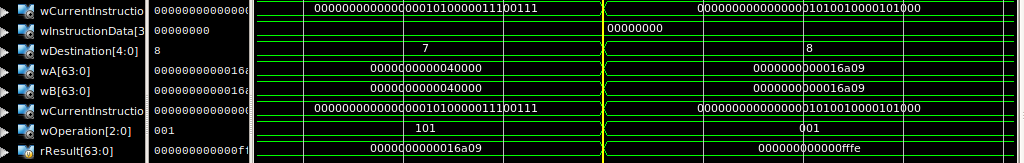
\includegraphics[width=1\linewidth, height=2.5cm]{images/Selection_010}
	\caption{Primera parte de captura de la simulación de señales} \label{fig:sim1}
\end{figure}

En la imagen 1 se pueden seguir viendo las operaciones que corresponden a los pasos intermedios de multiplicación por los que pasa.

En la imagen 2 se observa que después de realizar las operaciones de multiplicación, resta y desplazamiento se obtiene que en la última operación el registro rResult adquiere el valor de 0x16A0A, equivalente a 0.7071075, lo cual implica que la iteración respecto al valor ini mejoró la aproximación del inverso de la raíz cuadrada pues el valor real es aproximadamente 0.7071067. Lo anterior implica la tendencia de mejorar la precisión siempre y cuando se encuentre un valor inicial cercano al valor meta. 

\begin{figure}
	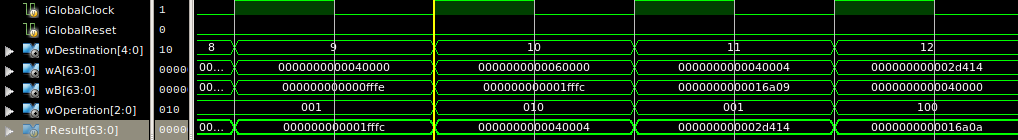
\includegraphics[width=1\linewidth, height=2.5cm]{images/Selection_011}
	\caption{Segunda parte de captura de la simulación de señales} \label{fig:sim2}
\end{figure}

\section{Pruebas en los distintos rangos de bits de entrada}

El  RGU inicialmente emplea números de 32 bits con 15 bits de parte entera. La parte entera de estos números se emplea como valor de entrada a una tabla de memoria con 128 valores (7 bits). La tabla de memoria está encargada de generar un valor de iteración inicial, por lo que se implementó un módulo llamado FixedPointSquareRoot cuya finalidad es aumentar el rango de cobertura de la RGU, pero dicho módulo aumenta el error al hacer una estimación ya que hace un corrimiento hacia la derecha de los 8 bits menos significativos de la parte entera de los números en punto fijo para poder encontrar un valor en la tabla que abarca solo números de 7 bits (128 posibilidades).

\begin{figure}
	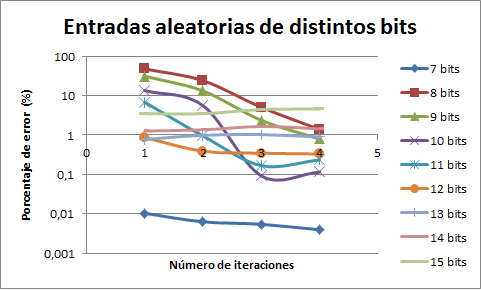
\includegraphics[width=0.7\linewidth]{images/puntos}
	\caption{Gráfico sobre los porcentajes de error ante iteraciones con distintos rangos de bits} \label{fig:puntos}
\end{figure}
En la tablas \ref{tab:errores1} y \ref{tab:errores2} y en la figura \ref{fig:puntos} cuya escala en el eje Y es logarítmica, se pueden observar que los porcentajes de error en 8 y 9 bits al iniciar las iteraciones eran bastante altos (de hasta 50 porciento) pero conforme se iteraba 6 y 7 veces se alcanzaba un porcentajes de error promedio inferiores a 0.05 porciento. 

En general la tendencia de las entradas con distintos bits es disminuir su porcentaje de error conforme se van aumentando las iteraciones. Solo en los casos de 14 y 15 bits se puede apreciar que se pierde el cáracter de disminución observado en los casos de menor cantidad de bits y más bien se genera un error casi constante, lo cual estaría dado por la incapacidad del hardware de proporcionar valores iniciales más precisos para lo cual se necesitaría tablas con mayor cantidad de valores, y de hecho los errores máximos en el caso de entradas de 15 bits llega casi el 10 porciento en promedio después de 7 iteraciones.
 
Sucede que en valores de entrada de solo 8 y 9 bits el error inicial es mucho ya que siempre se está haciendo un corrimiento de 8 bits a la parte entera del número en el módulo de FixedPointSquareRoot, y tal efecto se podría disminuir  al reducir el corrimiento de 8 bits a un corrimiento de 4 bits, lo cual implicaría correr la coma en los números en punto fijo de modo que haya 21 bits de parte fraccionaria y 11 bits de parte entera.


\begin{table}[htbp]
  \centering
  \caption{Tabla de iteraciones de 7 a 12 bits de entrada con su respectivo error}
    \begin{tabular}{rrrrrrrrrr}
    \toprule
    Iteración & 7     & 8     & 9     & 10    & 11    & 12 \\
    \midrule
    1     & 0,00841071 & 50,0658633 & 30,7774517 & 15,6596942 & 7,76805536 & 3,66909914  \\
    2     & 0,00894086 & 23,5363945 & 13,9400145 & 5,31296183 & 2,41015261 & 1,18594374  \\
    3     & 0,00930179 & 8,55821424 & 4,29449621 & 1,32698968 & 0,62065573 & 0,53281164  \\
    4     & 0,00876417 & 1,69111624 & 0,90878392 & 0,32663346 & 0,23015816 & 0,36576529  \\
    5     & 0,00706618 & 0,08517355 & 0,05935672 & 0,08746336 & 0,18863339 & 0,39944359  \\
    6     & 0,00716321 & 0,0177213 & 0,04125542 & 0,11741878 & 0,20503292  & 0,39260082   \\
    7     & 0,00864808 & 0,02467144 & 0,03124886 & 0,05765008 & 0,14925324 & 0,26242017  \\
    \bottomrule
    \end{tabular}%
  \label{tab:errores1}%
\end{table}%
% Table generated by Excel2LaTeX from sheet 'Hoja1'
\begin{table}[htbp]
  \centering
  \caption{Tabla de iteraciones de 13 a 15 bits de entrada con su respectivo error}
    \begin{tabular}{rrrrrrrrr}
    \toprule
    Iteración     & 13    & 14    & 15 \\
    \midrule
    1    &    3,21100282 & 2,83521291 & 3,69484261 \\
    2    &    1,58770231 & 1,77968444 & 3,06908    \\
    3    &    1,03472789 & 1,63220475 & 3,31805053 \\
    4    &    0,71357453 & 1,70383192 & 3,46803755 \\
    5	 &    0,67879743 & 1,52332552 & 3,10363742 \\
    6    &    0,8514918 & 1,43644598  & 3,41601461  \\
    7    &    0,81234608 & 1,30897039 & 3,25471677 \\
    \bottomrule
    \end{tabular}%
  \label{tab:errores2}%
\end{table}% 

\section{Pruebas con una tabla distinta}

En esta sección se creó una nueva tabla de aproximación con 128 valores de punto fijo, cada uno con 21 bits de parte decimal y 11 bits de parte entera.  

En esta ocasión se modificó el módulo SquareRoot de modo que la parte entera en punto fijo solamente se le hiciera un corrimiento hacia la derecha de cuatro bits si los cuatro bits más significativos eran iguales a cero. Después de la realización del corrimiento se evaluaba en la tabla las entradas cuyo rango de valores oscilaba entre 7 y 11 bits en las distintas corridas, la gráfica de las simulaciones se puede observar en la figura \ref{fig:puntos2}.

Así se realizaron corridas de hasta siete iteraciones del método de Newton-Raphson para valores de entrada de 7, 8, 9, 10 y 11 bits, con ello se crearon simulaciones que reflejan porcentajes de error mucho menores (inferiores 0.1 porciento) que los que existían anteriormente pues antes en rangos de ocho bits en la primer iteración habían errores de hasta el 50 porciento, la tabla de errores de estas simulaciones se puede apreciar en la tabla \ref{tab:erroresTable}. Los valores más bajos de porcentaje de error promedio se encuentra al iterar 6 veces en el método, lo cual implica 32 ciclos de reloj y el uso de 31 instrucciones. 

\begin{figure}
	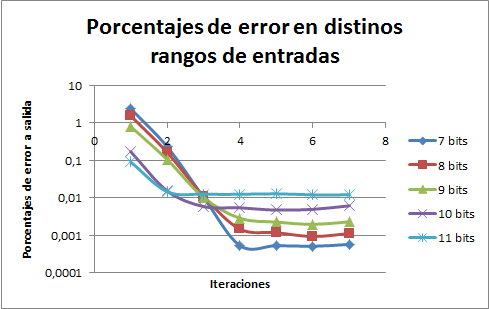
\includegraphics[width=0.7\linewidth]{images/puntos2}
	\caption{Gráfico sobre los porcentajes de error con una tabla distinta} \label{fig:puntos2}
\end{figure}

\begin{table}[htbp]
  \centering
  \caption{Tabla con errores}
    \begin{tabular}{rrrrrr}
    \toprule
    Iteración & 7     & 8     & 9     & 10    & 11 \\
    \midrule
    1     & 2,39768947 & 1,54218008 & 0,79985504 & 0,17164355 & 0,09036208 \\
    2     & 0,23224025 & 0,16369097 & 0,10533554 & 0,01536852 & 0,01459237 \\
    3     & 0,01037121 & 0,01102002 & 0,0102242 & 0,0058599 & 0,01255277 \\
    4     & 0,00052636 & 0,00146255 & 0,00283672 & 0,00541861 & 0,01242961 \\
    5     & 0,00052834 & 0,0011744 & 0,00224706 & 0,00469195 & 0,01280753 \\
    6     & 0,00050715 & 0,00092701 & 0,00196309 & 0,00492678 & 0,0120116 \\
    7     & 0,00057111 & 0,00111485 & 0,00229352 & 0,00612921 & 0,01204476 \\
    \bottomrule
    \end{tabular}%
  \label{tab:erroresTable}%
\end{table}%

%%%%%%%%%%%%%%%%%%%%%%%%%%%%%%%%%%%%%%%%%%%%%%%%%%%%%%%%%%%%%%%%%%%%%%%%%%%%%%%%%%%%%%%%%%%%%%%%%%%%%%%%%%%%
%%%%%%%%%%%%%%%%%%%%%%%%%%%%%%%%%%%%%%%%%%%%%%%%%%%%%%%%%%%%%%%%%%%%%%%%%%%%%%%%%%%%%%%%%%%%%%%%%%%%%%%%%%%%
%%%%%%%%%%%%%%%%%  MACHOTE  %%%%%%%%%%%%%%%%%%%%%%%%%%%%%%%%%%%%%%%%%%%%%%%%%%%%%%%%%%%%%%%%%%%%%%%%%%%%%%%%
%%%%%%%%%%%%%%%%%%%%%%%%%%%%%%%%%%%%%%%%%%%%%%%%%%%%%%%%%%%%%%%%%%%%%%%%%%%%%%%%%%%%%%%%%%%%%%%%%%%%%%%%%%%%
%%%%%%%%%%%%%%%%%%%%%%%%%%%%%%%%%%%%%%%%%%%%%%%%%%%%%%%%%%%%%%%%%%%%%%%%%%%%%%%%%%%%%%%%%%%%%%%%%%%%%%%%%%%%
\begin{comment}


\section{Pruebas para comprobar la funcionalidad y estabilidad}

Al finalizar el desarrollo de la aplicación, se probó acceder a ella desde computadoras en diferentes sistemas operativos. En todos los casos la aplicación operaba de forma correcta. Por lo que independientemente del OS del sistema, la herramienta es funcional, dando como resultado una aplicación web, multiplataforma. Lo cual era uno de los objetivos que se quería alcanzar inicialmente.\\

Además se analizó la exactitud de los datos obtenidos. A la hora de realizar los contornos con la herramienta desarrollado, siempre se obtuvo todos los pixeles que forman parte del mismo, distinto a Sensarea que se obtenían muy pocos puntos si se realizaba la funcionalidad de esta misma manera (dejando precionado el click izquierdo y desplazando el puntero al rededor del contorno).


\section{Pruebas realizadas por diversos usuarios}

Para probar que la aplicación diseñada en efecto es más sencilla de utilizar que las otras herramientas actuales y que con ella se generan datos de manera más eficiente, se procedió a realizar unas pruebas con tiempo a tres diferentes usuarios y se promedió el resultado. Las otras dos herramientas con las cuales se comparó fueron Sensara y VideoANT, debido a que son las únicas que no se requiere de conocimiento técnico para poder instalarlas o utilizarlas en línea. A cada uno se les solicitó realizar las siguientes tareas en orden:

\begin{enumerate}
\item Instalar o acceder a la aplicación
\item Abrir la aplicación, cargar uno de sus video y realizar la segmentación temporal de 5 escenas diferentes.
\item Seguir de la trayectoria de 5 elementos diferentes por al menos 20 cuadros.
\item Dibujar los contornos de 5 elementos diferentes por al menos 20 cuadros.
\item Realizar anotaciones semánticas de 5 tipos diferentes de escenas encontradas.
\end{enumerate}

El video que se utilizó fue una sección de la final de la Copa del Mundo Fifa 2010 entre España y Holanda. El peso del video es de 250 Mb, el formato es mp4 y codec es h264. Los resultados obtenidos se muestran en las tablas \ref{table:results} y \ref{table:results2}. La primera de ellas muestra lo que se duró haciendo la labor por primera vez y en la segunda tabla se muestra el valor promedio de tiempos en las 5 tareas de cada tipo.


\begin{table}[h]\centering
	
	\ra{2}
	\caption{Promedio de tiempo estimado de la primera función realizada correctamente}
	\label{table:results}
	
	\begin{tabular}{@{}cC{3cm}C{3cm}C{3cm}C{3cm}c@{}}\toprule
		
		& Función & GT-Tool & Sensarea & VideoANT&\\ \midrule
		
		& Primer uso de la aplicación & 7 segundos* & 2 minutos & 5 segundos* & \\
		
		& Segmentación temporal  & 26 segundos & 87 segundos & 15 segundos & \\
		
		& Rastreo de objetos & 5 segundos & 5 segundos & no aplica & \\
		
		& Segmentación de contornos & 27 segundos  & 34 segundos & no aplica & \\
		
		& Segmentación semántica & 20 segundos  & no aplica & 15 segundos & \\ 
		
		\bottomrule
		
	\end{tabular}
	
\end{table}

*Ese el tiempo que les tomó acceder a la página web, de lo contrario es el tiempo de descarga e instalación.\\

Se puede apreciar de esta primera tabla (\ref{table:results}), que GT-Tool es muy similar a Sensarea cuando se quiere realizar el seguimiento de la trayectoria de los objetos. Y es un poco más lento que VideoANT a la hora de realizar la segmentación temporal y semántica, esto es debido a la forma en la que VideoANT solicita la información, es más directa pero no tan especializada. De nuevo, VideoANT da precisión de segundos y no de cuadros y además no tiene manera de realizar seguimiento de trayectorias ni segmentación de contornos.\\

A continuación el promedio de las 5 repeticiones luego de haber realizado la tarea por primera vez:


\begin{table}[h]\centering
	
	\ra{2}
	\caption{Promedio de tiempo que tomó realizar cada función repetidas veces (5 repeticiones)}
	\label{table:results2}
	
	\begin{tabular}{@{}cC{3cm}C{3cm}C{3cm}C{3cm}c@{}}\toprule
		
		& Función & GT-Tool & Sensarea & VideoANT&\\ \midrule
		
		& Segmentación temporal  & 19 segundos & 30 segundos & 13 segundos & \\
		
		& Rastreo de objetos & 3 segundos & 4 segundos & no aplica & \\
		
		& Segmentación de contornos & 14 segundos  & 29 segundos & no aplica & \\
		
		& Segmentación semántica & 15 segundos  & no aplica & 13 segundos & \\ 
		
		\bottomrule
		
	\end{tabular}
	
\end{table}

Al analizar los resultados de dicha tabla se concluye los siguiente:

\begin{enumerate}
	
\item A medida que utilizan cualquier herramienta, el tiempo que les toma realizar una labor disminuye, sin importar cual sea. La disminución más grande la tuvo Sensarea en la segmentación temporal, pero esto fue debido a que, aunque Sensarea no soporta nativamente algún tipo de segmentación temporal, se puede simular colocando puntos con etiquetas. Cuando los usuarios se dieron cuenta de esto, lo empezaron a hacer y así hacían un tipo de segmentación temporal.

\item VideoANT continua siendo un poco más rápida para lo temporal y semántico, pero no cuenta con los otros tipos. De igual manera la diferencia en tiempos no es muy significativa.

\item GT-Tool si logra disminuir el tiempo en el que se generan los datos para la trayectoria de objetos y segmentación de contornos, mientras que a la vez aumenta la precisión brindada por Sensarea.

\end{enumerate}

\end{comment}
	
	%conclusiones
	%\chapter{Conclusiones y recomendaciones}

Para finalizar este informe escrito, se expone las conclusiones, se da algunas recomendaciones y se propone trabajo que queda aún por realizar para seguir perfeccionando la herramienta. Las conclusiones se realizan con relación directa a los objetivos tanto el general como los específicos propuestos al inicio del trabajo y los resultados obtenidos luego de la creación de la aplicación y el uso de la misma.

\section*{Conclusiones}

\begin{itemize}
	
\item Se concluyó satisfactoriamente la creación de una aplicación web para la generación de los 4 diferentes tipos de segmentación requeridos: temporal, trayectorias, contornos y semántica. La aplicación es completamente funcional, permite cargar videos locales, guardar y cargar proyectos, y descargar los datos generados en formato JSON para poder procesarlos y compararlos con los datos que son obtenidos de los algoritmos.

\item El cargar videos desde el servidor se vio limitado a la funcionalidad que tienen los navegadores en la actualidad. Estos no están hechos para cargar todo el video rápidamente y poder manipular su tiempo tan deliberadamente, los videos en \emph{streaming} en los navegadores están diseñados para utilizar el mínimo ancho de banda posible y la principal función del navegador es reproducirlo una sola vez, por lo que no carga todo como es necesario y además va limpiando el \emph{buffer} de carga, por lo que los datos que se tenían cargados previamente, si ingresan muchos datos, son desechados y no se puede regresar a esas secciones del video sin volver a realizar un \emph{buffering} desde cero.

\item Las herramientas web disponibles en la actualidad satisfacen diferentes necesidades y diferentes gustos según el programador. En distintos lenguajes de programación como en Python y JavaScript, con diferentes tipos de servidores sincrónicos o asincrónicos. Quedará siempre a criterio del ingeniero que tipo de herramienta le es más útil dados sus gustos y el tipo de aplicación que quiere llegar a tener al final.

\item Se diseñó correctamente una base de datos del tipo NO-SQL, utilizando MongoDb. Esta base de datos tiene la ventaja de que escala rápidamente, que su formato de lectura y escritura predeterminado es JSON, el cual se utiliza ampliamente en los frontend en JavaScript o Python, lo que convierte a MongoDb en una excelente opción en bases de datos no relacionadas para aplicaciones o sitios web que se basen en estos lenguajes de programación.

\item Los resultados de comparar el uso de GT-Tool con Sensarea y VideoANT comprueban que se logró realizar una herramienta más eficiente en todos los aspectos a evaluar. Los datos de trayectoria y contorno se generan más rápido y con una resolución de puntos mayor para poder validar de mejor manera los algoritmos. En el caso de la segmentación temporal y semántica no es más rápida que VideoANT, pero esto se compensa ya que GT-Tool si logra realizar esta segmentación a nivel de cuadros y no de segundos como lo hace VideoANT. Además GT-Tool tiene de forma nativa e intuitiva el como realizar cada uno de los tipos de segmentación, y es una solución multiplataforma.

\item Se creó satisfactoriamente un manual básico y fácil de entender para que los usuarios puedan instalar y hacer uso de la herramienta correctamente y en poco tiempo. Además el video tutorial está disponible en línea en  \url{pris.eie.ucr.ac.cr/tools/gt-tool}.

\end{itemize}

\section*{Recomendaciones}

\begin{itemize}
	
	\item El desarrollo de software, especialmente de aplicaciones completas, es una tarea bastante complicada, más si todas las labores las realiza una sola persona. Se recomienda tener un equipo de más personas debido a que hacer el diseño de la interfaz gráfica, el desarrollo de funcionalidades y la verificación de las mismas, todo por una sola persona, con lleva mucho tiempo y no es lo ideal, ya que no se toma en cuenta lo que piensan otras persona de la interfaz y algunos errores se pasan por alto porque otra persona usó exhaustivamente la aplicación.
	
	\item En este tipo de diseños es importante asegurar que el código es legible para poder darle mantenimiento en presencia de cualquier problema. Es importante llevar una buena documentación a lo largo de todo el desarrollo ya que ayuda a mantener el orden y a entender mejor las labores que se está realizando.
	
	\item Seguir patrones de diseño como el MVC es de gran utilidad en el desarrollo de aplicaciones. Le da características modulares al código, por lo que si se quiere cambiar la interfaz del programa, se puede alterar únicamente los valores y archivos de los objetos que tienen que ver con los Views y los demás pueden mantenerse igual. Si todo se realiza correctamente la compatibilidad entre la nueva interfaz y el código de controllers y model anterior debe de funcionar en su totalidad o por lo menos con una compatibilidad muy alta.
	
\end{itemize}

\section*{Trabajo por realizar}

En vista de que un software nunca alcanza su versión final, siempre hay errores que se pueden reparar, desempeño que se puede mejorar o funcionalidades que se pueden agregar, se tiene una lista de funcionalidades o extras que pueden ser muy útiles de tener en la aplicación:

\begin{itemize}
\item Una plantilla en formato tipo JSON que se pueda cargar a los diferentes modos para personalizar el nombre de las etiquetas de la segmentación temporal o configurar previamente la cantidad de contornos o trayectorias y sus colores en los respectivos modos de operación.

\item Desarrollar alguna solución para poder cargar videos del servidor en su totalidad sin perder el buffering anterior o poder adelantarlo si se quiere cargar solo una sección adelantada del video.

\item La implementación de comandos comunes del teclado utilizados en la mayoría de software. Por ejemplo ctrl-z para deshacer y ctrl-s para guardar.

\item Crear una aplicación para dispositivos móviles que utilice la misma base de datos.

\item Instalar la aplicación en un servidor y realizar pruebas de estrés y carga por cantidad de usuarios y peticiones.

\item Ofrecer la posibilidad de descargar los datos generados en diferentes formatos: JSON, YAML, XML, entre otros.

\end{itemize}
	
	%--------------------------------------------------------------------
	%bibliografía
	\bibliography{eieclases}
		
	\cleardoublepage
	
	%--------------------------------------------------------------------
	%apéndice
	\appendix
	
	%\include{apendice0}
	%\include{apendice1}
	%\include{apendice2}
	
	%final del documento
\end{document}
